% \listfiles
\documentclass[a4paper]{article}
\usepackage[T2A]{fontenc}
\usepackage[english,russian]{babel}
\usepackage{sectsty}
\sectionfont{\centering\normalfont}
\subsectionfont{\centering\normalfont}
\subsubsectionfont{\normalfont}
\usepackage{changepage}
\usepackage{filecontents}
% \usepackage{mathptmx}
\usepackage{float} 
\usepackage{subcaption}
\usepackage[utf8]{inputenc}
\usepackage[14pt]{extsizes}
\usepackage{physics} 
\usepackage{graphicx}
\usepackage{enumerate}
\graphicspath{{../misc/}}
\usepackage{setspace,amsmath}
% \usepackage[left=30mm, right=15mm, top=20mm, bottom=20mm]{geometry} 
\usepackage[nottoc]{tocbibind}
\usepackage[style=gost-numeric,sorting=none,backend=biber,defernumbers=false]{biblatex}
\DeclareBibliographyAlias{misc}{article}
\addbibresource{lit.bib} 
%%%%%%%%%%%%%%%%%%%%%%%%%%%%%%%%%%%%%
% \everymath{\displaystyle}
\DeclareMathSizes{12}{20}{14}{10}

\makeatletter
\def\@makefnmark{\hbox{\@textsuperscript{\normalfont(\@thefnmark)}}}
\makeatother
 
\captionsetup[figure]{labelsep=period}
\captionsetup[table]{labelsep=period}

\usepackage{titling,lipsum}

\usepackage{amsmath}
\usepackage{bm}

\usepackage{hyperref}
\hypersetup{
    colorlinks,
    citecolor=black,
    filecolor=black,
    linkcolor=black,
    urlcolor=blue
}

\begin{document}

\thispagestyle{empty}

\begin{center}
    \large\textbf{Training competition connections between local receptive fields in spiking neural networks}\\
    \hfill\break
    
    Daniil Gafni, Dmitry Nekhaev, Vyacheslav Demin
\end{center}


% \tableofcontents


% \pagebreak

\addcontentsline{toc}{section}{Abstract}
\section*{Abstract}
Standard learning methods (based on the error backpropagation) used in formal artificial neural networks (ANNs) are difficult to apply to spiking neural networks (SNNs) due to discrete and time-distributed nature of the events they generate --- impulses, or spikes. Although such projects exist, local learning algorithms, which are more biologically correct, capable of performing unsupervised learning (without a teacher) and more energy efficient (if implemented on specialized hardware), are of greater interest.

One of the main disadvantages of the SNNs in comparison with the ANNs is the current understudy of local learning rules, and because of this, lower quality metrics (on inference) of algorithms based on SNNs. Thus, the study of SNN learning algorithms, like spike-timing-dependent-plasticity (STDP), for use in various SNN architectures is an important task.

The introduction of competition connections (having negative weights) allows to achieve a better distinction of features learned by the neurons. The most common way to introduce competition between SNN neurons is to use a group of winner-take-all methods, where the first neuron in the layer that generates an impulse either zeroes the membrane variables of other neurons or prohibits other neurons from generating spikes for a given time. The use of competition connections in the form of negative synaptic weights has not been studied either, and the influence of the possibility of updating them according to local rules, along with stimulating projections, has been hardly studied too. In this work, it is shown that learning competition relationships in the architecture of a locally connected SNN potentially allows to achieve better results in the accuracy of pattern recognition (on MNIST digits) due to the organization of competitive and at the same time cooperative work of groups of neurons.

\pagebreak

\addcontentsline{toc}{section}{Introduction}
\section*{Introduction}

Modern formal neural networks do an excellent job at solving many machine learning problems \cite{pmlr-v28-wan13, Khan_2020}. However, training them is a laborious process that requires large computational resources. Typically, training is conducted using hundreds or thousands of examples and can take months. Both training and inference of formal neural network algorithms are far from being effective \cite{Edwards2015GrowingPF}. This is due both to the physically separate storage of connection weights and neuron activations, and to the calculations themselves, which are tensor in nature, associated with vector-matrix and matrix-matrix multiplication of floating point numbers. Modern CPUs are not optimized for this kind of computing. GPUs --- architectures originally created for working with computer graphics, and therefore more suitable for tensor calculations --- are much better at these tasks than traditional CPUs, but they do not perform with the desired efficiency either. The number of parameters in modern formal neural networks can reach tens \cite{ManyParams, Khan_2020} and even hundreds of billions (the latest OpenAI language model GPT-3 \cite{brown2020language}).

Spiking neural networks (SNNs) are an alternative promising neuromorphic algorithm and have several advantages over formal neural networks.

\begin{itemize}
\item SNNs allow a richer dynamic coding of patterns in continuous time, which is usually not available for formal neural networks \cite{Ismail_Fawaz_2019}. Thus, SNNs are of greatest interest for solving time series problems (video and sound streams processing, speech recognition, decision making).

\item Local algorithms, which use only information from the neurons connected by this connection to update the weight of each connection \cite{STDP, pehlevan2019spiking, Baldi_2016}, can be used to train SNNs. On the contrary, when training formal neural networks, information about all neural connections between this connection and the output of the network is used to update the weight of each connection. Thus, SNNs learning algorithms on their own are far more efficient than formal neural network learning algorithms.

\item Moreover, these algorithms can use unsupervised learning, which does not require manual data labeling, as in the case of backpropagation methods.

!!!!!!!!!!!!!!!!!!!! TODO: find references below

\item SNNs can be implemented on specialized neuromorphic processing units (both based on digital elements \cite{TrueNorth, Loihi, Akida} and using hybrid digital-analog circuits (BrainScales, \cite{SpiNNaker}), including those based on memristors [links to others (Ielmini, Querlioz) and our works]), which have ultra-low power consumption (achieved by reducing the number of acts and the average length of signal transmission, as well as the spatial and temporal sparseness of spikes in the network). This implementation, together with the algorithmic advantage of the SNNs, also provides significant performance gains. \cite{hardware1, hardware2}.

\item SNNs, to a greater extent than formal neural networks, biologically correctly model the interactions of neurons, which can be used for biological simulations of the nervous system for the purposes of studying not only bioinformatics, but also biophysical and medical aspects of its functioning.
\end{itemize}

It is of interest to study well-known ANN architectures in application to SNN, such as convolutional, locally connected and fully connected \cite{Khan_2020} architectures. Moreover, the introduction of additional recurrent competition connections contributes to a better separation of features in the learning process \cite{MaxActiv1, MaxActiv2}. A fully connected network is the simplest model that can be used as a benchmark. Convolutional and locally connected architectures use convolution --- an operation that allows to extract important features more efficiently (comparing to a fully connected network). The locally connected architecture is especially interesting, because it can be easily implemented in hardware, since, unlike a convolutional network, it does not use shared synaptic weights  inside a separate feature map. A locally connected architecture has significantly fewer parameters than a fully connected architecture and allows to train a unique set of features for each receptive field, in contrast to convolutional networks. At the same time, convolutional networks have translational invariance, a useful property for image processing (spatially correlated data). The presence of competition in the SNN makes it possible to make their features more independent. Therefore, for experiments in this work, we chose locally connected SNNs with competition links, and as basic models, convolutional and fully connected networks with competition connections:

\begin{enumerate}[i]
\item we study the effect of training the competition connections \cite{MaxActiv1, MaxActiv2, hardware_survey} between neurons on the accuracy of the image classification problem of handwritten digits from the MNIST \cite{MNIST} dataset for the architecture of a locally connected network (Locally Connected Spiking Neural Network, LCSNN) \cite{saunders2019locally};

\item compare this architecture with a Convolution Spiking Neural Network (CSNN) and a Fully Connected Spiking Neural Network (FCSNN).
\end{enumerate}

\clearpage

\section{Training of the SNN with fixed competition connections of local receptive fields}

\subsection{Problem description}
For the comparative analysis, a classical machine learning problem was chosen --- the problem of classifying images of handwritten digits from the MNIST dataset. MNIST consists of labeled training and test subsets of 60,000 and 10,000 images. The images have 28 $ \times $ 28 resolution and are black and white. Due to the need to calibrate the networks (see below), the original training subset was split into 50,000 images for training (training dataset) and 10,000 images for calibration (calibration dataset).

The images are also cropped so that only the center 20 $ \times $ 20 pixels are used. \\

\subsection{Competition between local receptive fields in SNN}
In this paper, networks are studied using locally connected, fully connected and convolutional layers. In a fully connected layer, each neuron is connected to each neuron from the previous layer. In the convolutional layer, neurons are divided into channels. The neurons in one channel have shared weights, but each neuron is only connected to a certain region (rectangular in the case of a two-dimensional layer) \cite{li2020survey} --- receptive field, or patch. The architecture of the locally connected layer is the same, but each neuron has its own unique weights \cite{saunders2019locally}.

The neural network architecture of LCSNN is inspired by the structure of the visual cortex of the brain. The $Y$ network layer consists of $n$ channels, each of which is locally connected to the $X$ layer of neurons. We connect neurons with common receptive fields by competition connections.

\begin{figure} \label{LCSNN}
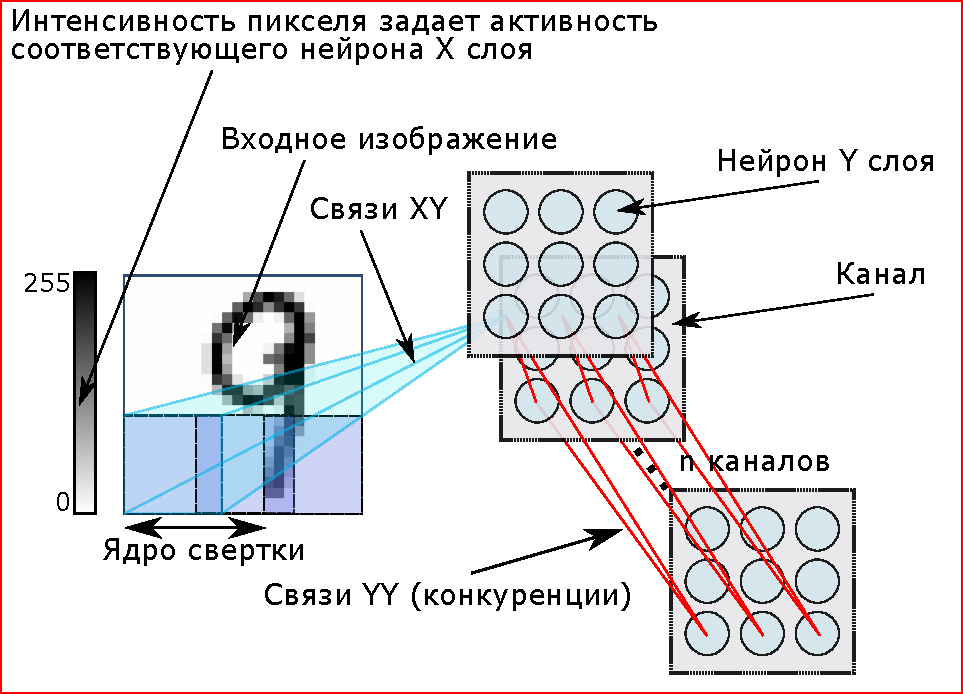
\includegraphics[,
 width=\textwidth,keepaspectratio=true]{LCSNN_ru.pdf} 
    \caption{LCSNN architecture}
\end{figure}

Such connections have negative weights, which means they negatively affect neuron activity. Neurons that do not have a common patch (and therefore respond to different areas of the image) do not compete with each other. Competition connections are introduced to improve the separation of neurons by learned features. A similar architecture can be built for networks with convolution or fully connected layers. We studied networks with the number of $Y$ neurons $\approx$ 100 --- 900 and folowwing convolutions parameters: kernel size of 8 or 12 and stride of 4. Since the MNIST images were cropped to a size of 20 $\times 20$, the number of neurons per the channel was 3 or 4.

This work uses the Adaptive Integrate-And-Fire (ALIF) model of neurons. The dynamics of the neuron potential in this model is given by the equation

\begin{equation} \label{eq:alif}
 \tau_v \dv{v(t)}{t} = -v(t) + v_{rest} + I(t) \cdot R \text{,}
\end{equation} where $I(t)$ is the current, accumulated by time moment $t$, $v_{rest}$ --- relaxation level, $\tau_v$ --- simulation time constant, а $R$ --- unit coefficient, numerically equal to one.\\ 

Activation threshold $v_{thresh}$ of an ALIF neurone is not static, but slightly increases with every spike, then relaxing to its initial value $\theta_o$. The dynamics of the activation threshold is given by:
\begin{equation} 
 v_{thresh} = \theta_0 + \theta(t) \text{,}
\end{equation} where $\theta_0$ is the initial activation threshold, $\theta(t)$ --- an adaptive additive to the activation threshold after each spike generation, which is calculated from the condition\\

\begin{equation}
 \tau_v \dv{\theta(t)}{t} = -\theta(t)
\end{equation}\\

After the generation of each spike, a short refractory period occurs, when for time $t_{refract}$ the potential of the neuron remains at the level of $v_{reset}$. The initial connection weights are generated randomly from a uniform distribution.

\subsection{Forward connections training}
To reduce the number of model parameters, images are cropped to 20 $\times$ 20 pixels. The edges of the images are often almost empty, so this operation has little or no effect on the amount of information, available to the network. For each image, $X$ spikes are generated using a Poisson distribution with a mathematical expectation value  proportional to the corresponding pixel intensiveness. Connections $XY$ are trained according to the STDP \cite{STDP} rule. This is a biologically inspired rule of unsupervised learning. When the presynaptic spike (pre-spike) is received and the post-spike is emitted, the weight $w$ of the corresponding connection is increased by $ \Delta w $, where
\begin{equation} 
\Delta w =
 \begin{cases}
 A_+ \cdot e^{- \frac{t_{pre} - t_{post}}{\tau_+}}, t_{pre} - t_{post} > 0\\
 A_- \cdot e^{- \frac{t_{pre} - t_{post}}{\tau_-}}, t_{pre} - t_{post} < 0
 \end{cases}
\end{equation}

Let's notice, that

$$
\begin{cases}
 A_{+} > 0\\
 A_{-} < 0
\end{cases}
$$

Thus, in the process of learning, the weights of connections where pre-spikes are systematicly recieved right before the emmision of post-spikes are increased, and decreased if vice versa. After such training, the neurons begins to actively react to pre-spikes received from neurons with larger connection weights. If these pre-spikes are recieved in a short enough time period, they might cause a new spike. The opposite rule (with $A_{+}$ and $A_{-}$ having the opposite signs) is called the anti-STDP \cite{anti-STDP} rule. In this paper it is used to train competition conenctions.

After each training iteration, the weights are normalized to keep their sum equal to a certain constant. This is done to forbid the weights to grow too large. The value of the normalization constant is an important model hyperparameter that has to be carefully selected for each specific network architecture.

\begin{figure}
\centering
\begin{subfigure}{0.45\textwidth}
    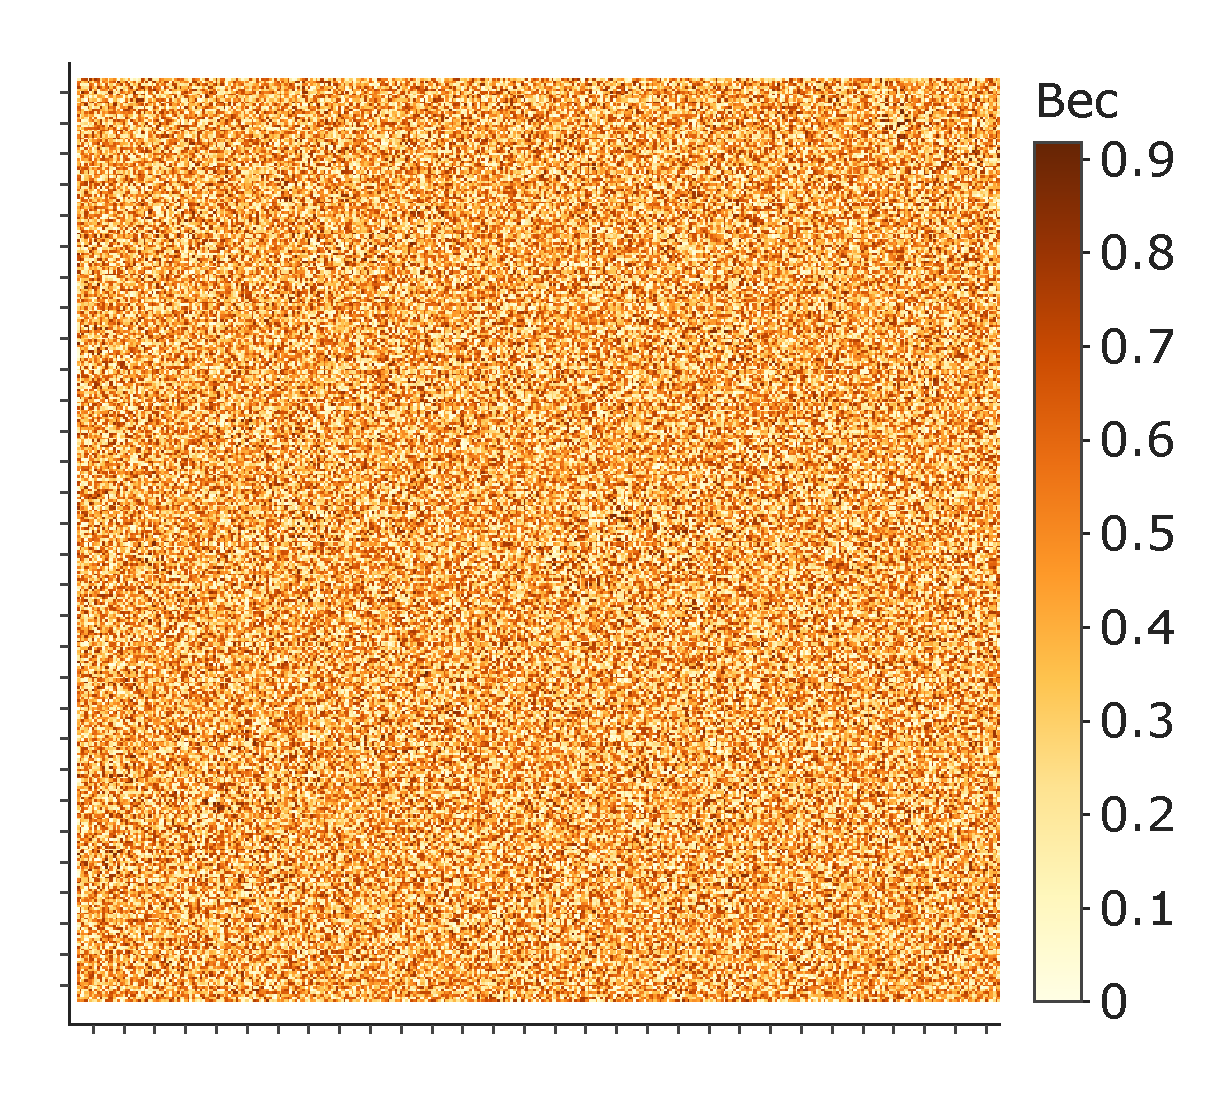
\includegraphics[width=\textwidth,keepaspectratio=true]{weights_XY_untrained_ru.pdf}
    \caption{Before training}
\end{subfigure}
\begin{subfigure}{0.45\textwidth}  \label{weights_XY}
    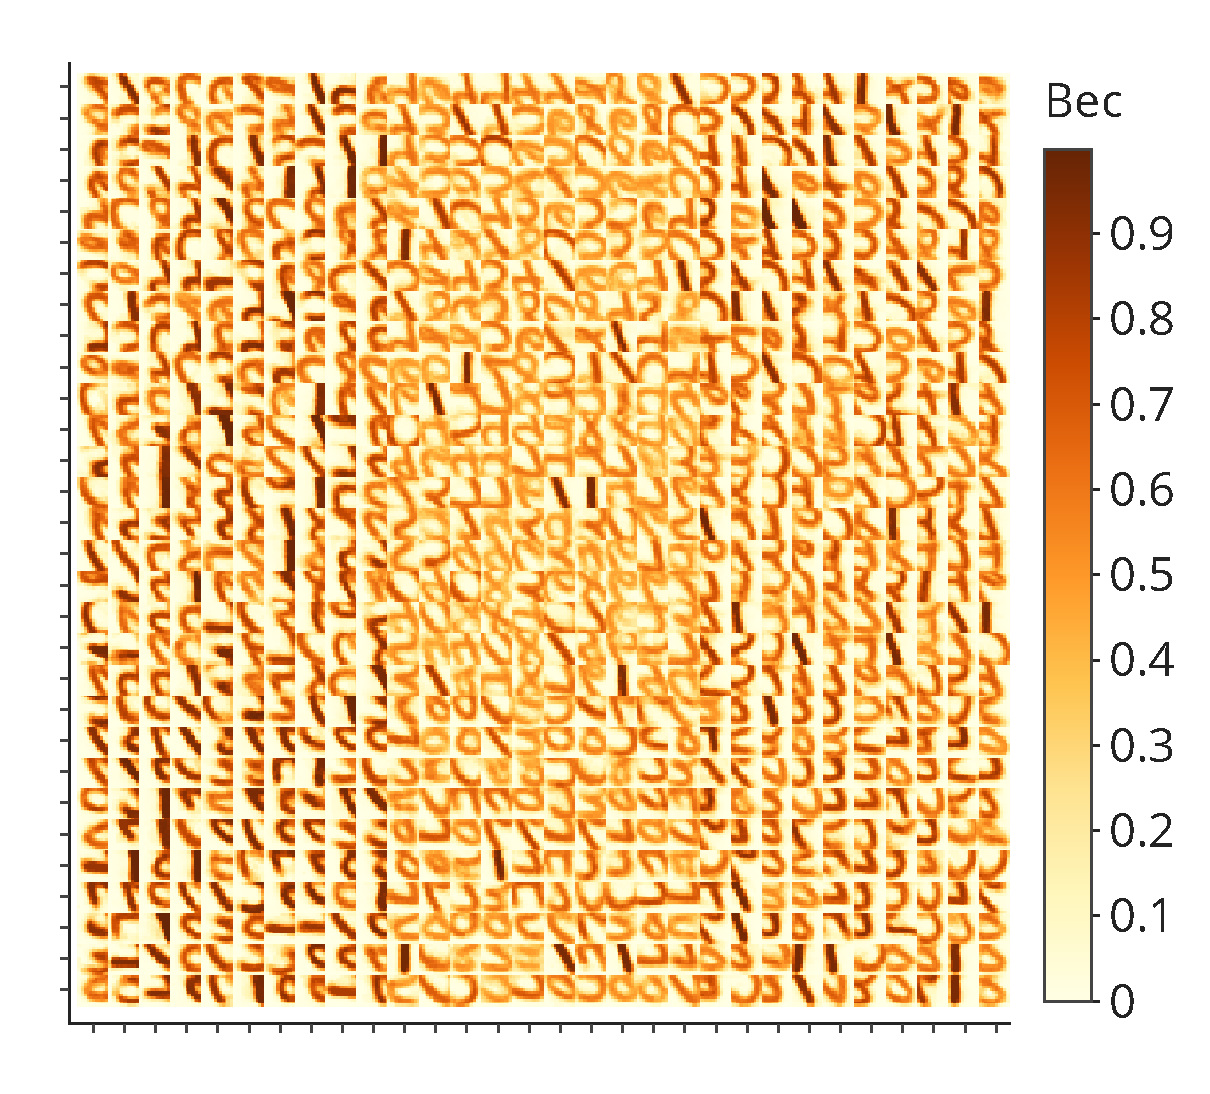
\includegraphics[width=\textwidth,keepaspectratio=true]{weights_XY_ru.pdf}
    \caption{After 1000 training iterations}
\end{subfigure}
\caption{Visualization of $XY$ connection weights of a 900 $Y$ neurons (100 neurons for each of the 9 patches) network --- a 360 $ \times $ 360 matrix. The weights of one neuron correspond to a 12 $\times$ 12 square. The weights of the $Y$ neurons are grouped by patch - the lower left 120 $  \times $ 120 square  (10 $ \times $ 10 neurons) corresponds to the lower left patch, the center square corresponds to the center patch, and so on. It can be seen that after training, the neurons learn features where digits elements can be observed.}
\end{figure}

\subsection{Spiking neural network activity interpretaion}

Several methods were used to interpret the activity of neurons in the $Y$ layer (that is, to correlate their activity with a certain class of recognizable digits): \textbf{patch voting}, \textbf{global voting}, \textbf{preselection by spikes voting} or a \textbf{linear classifier}. The first three methods have the advantage of being simple. However, the linear classifier significantly outperforms them in performance. \\

For the first three methods, it is necessary to calibrate the <<votes>> of neurons. Each neuron of the $Y$ layer is assigned 10 numbers (votes) for each digits class (from 0 to 9). The neuron-digit vote is calculated as the average number of spikes produced by the neuron in responce to the observation of this digit images by the network (throughout the entire time of the simulation) ---
$$ vote_i = \frac{\sum_ {1}^{n_{i}}{\sum_{0}^{t_{max}} s_t}} {n_{i}} \text {,} $$
where $ s_t $ takes the value 0 or 1 depending on the presence of a spike at a given time, $ n_i $ is the size of the calibration sample for the digit $ i $ (we used $ n_i = 1000 $).

For all networks, this calibration process was used for 10,000 examples from a calibration sample especially selected from the test part of the MNIST dataset, as noted above. Note that calibration is nota  part of the network training, since it is only included in the algorithm for interpreting the behavior of the SNS. The votes are used as a measure of confidence of the neuron in each of the digits classes.

\begin{figure}
\centering
\begin{subfigure}{\textwidth}
    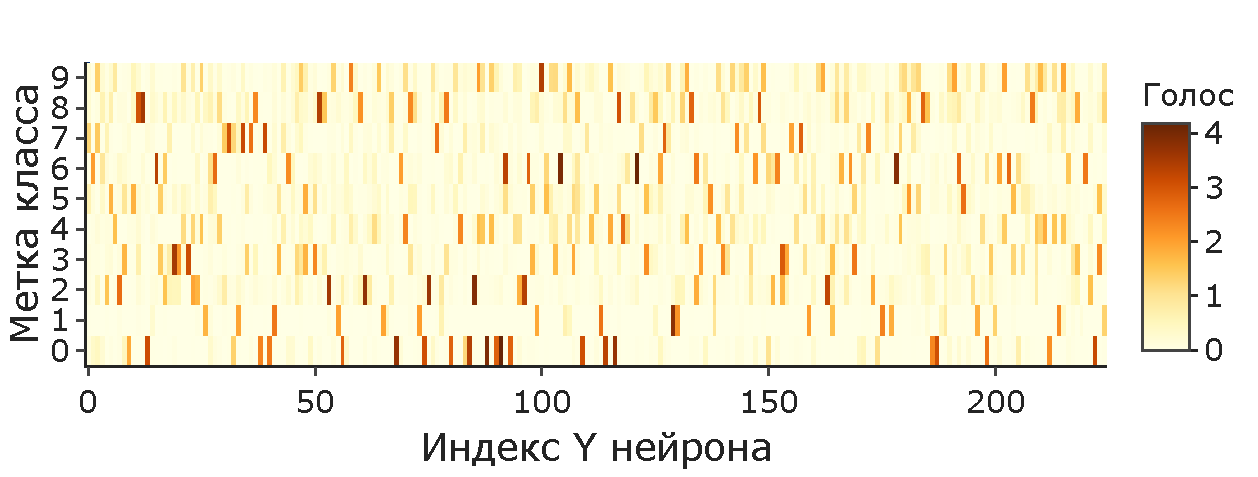
\includegraphics[width=\textwidth,keepaspectratio=true]{votes_ru.pdf}
    \caption{$Y$ neurons votes.}
\end{subfigure}
\begin{subfigure}{\textwidth} 
    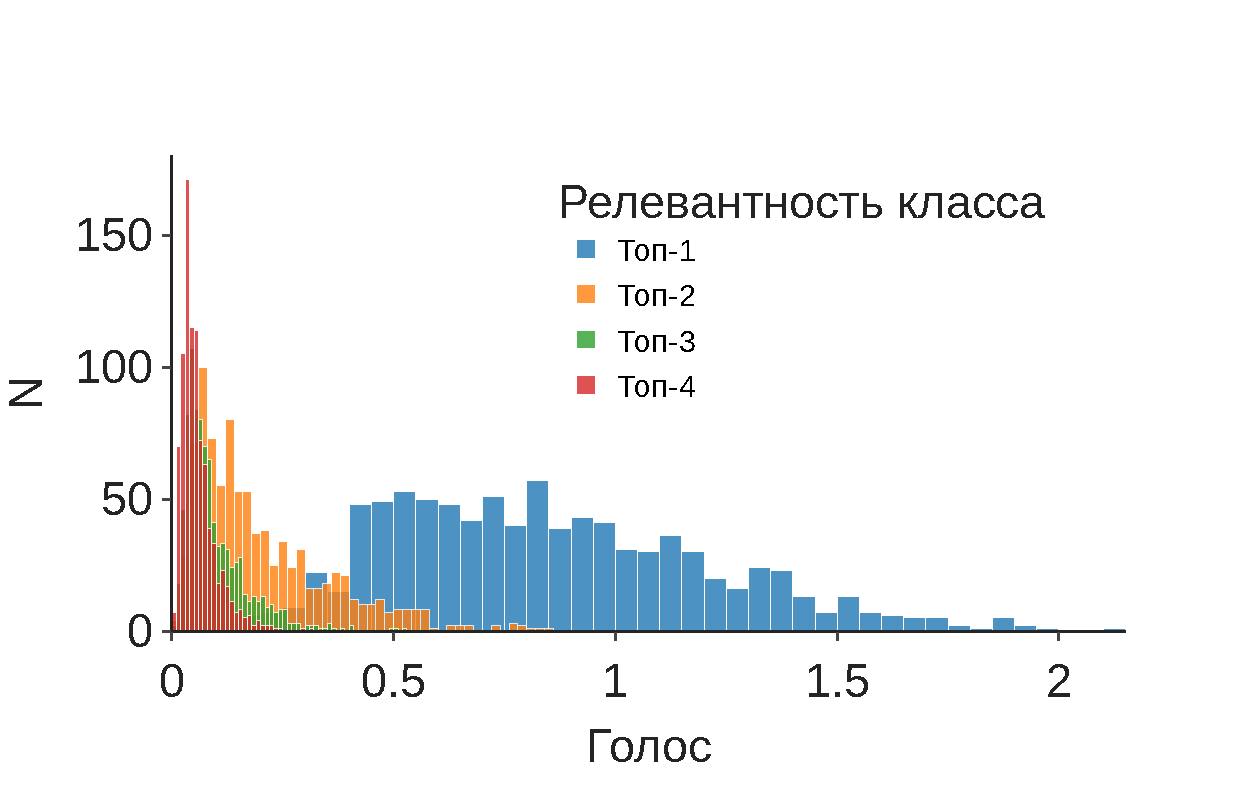
\includegraphics[width=\textwidth,keepaspectratio=true]{votes_distr_4_ru.pdf}
    \caption{Votes distrivution for the 4 most relevant classes (for each neuron). It can be seen that the vote value (average number of spikes per class) drops significantly with relevance decreasing.}
\end{subfigure}
\caption{Visualization of the votes of the $ Y $ network layer with 225 $ Y $ neurons. High values correspond to a large specialization of the neuron in the digits class. It can be seen that almost all neurons have a nonzero vote value, therefore, almost all neurons in the network are active.}
\end{figure}

Further, the product of the number of neuron spikes by its vote will be called \textit{score}.

In \textbf{global voting}, the network's response is considered to be the class with the highest \textit{score} among all neurons.

In \textbf{patch voting} the network response is considered to be the class with the highest \textit{score} among neurons with the highest \textit{score} per patch --- similiar to a maxpool operation in ANNs.

\textbf{Preselection by spikes voting} is done in a similiar fassion, but comparing the number of spikes, not \textit{scores}.

When using a \textbf{linear classifier}, the sums of spikes of individual  $ Y $ layer neurons are fed as features to te classifier, which is trained to predict the true image labels. As in other methods of interpreting the network activity, classifier training is performed on a separate calibration sample.

To evaluate the interpretation algorithm, accuracy is used - the ratio of the number of correctly recognized objects from a test sample to the size of the test sample. In this work, the test sample size (when measuring the accuracy for individual networks) is 10,000.

Accuracy learning curves were built for various interpretation algorithms. The accuracy was measured every 250 training iterations. To calibrate the interpretation algorithm at each step a calibration sample of 5000 was used, while to measure the accuracy, a test sample of 1000 was used.

After several thousand training iterations, the accuracy reaches a plateau. It is also noticeable that the three voting methods have very similar accuracy, while the linear classifier performes significantly better. The accuracy of even an untrained network can reach 70\% due to the fact that even with random weights initialization, different feature maps are formed, with some being a little better at recognizing certain patters, which can be amplified by the interpretaion alrorithm. It is known from \cite{saunders2019locally} that for a sufficiently large number of parameters, a locally connected network outperforms a convolutional and fully connected network in learning speed, since more parameters are updated with each training iteration (at least one neuron per patch is active). In the present study, no such effect is observed, since the presented learning curves are constructed for insufficiently large networks. Interestingly, the use of a linear classifier does not improve the recognition accuracy for a fully connected network - most likely due to the selection of voting features throughout the image, in contrast to convolutional and locally connected architectures.

The linear classifier surpasses the LCSNN- and CSNN-based voting algorithms in accuracy, since it is a generalization of voting in the sense that it also uses the sum of the products of weights/votes by neurons activity. However, when training a linear classifier effective optimization algorithms (including gradient) are being used, while when voting we achieve practically the same goal (calculating satisfactory votes/weights) with a heuristic - the averaged activity of neurons by classes.

\begin{figure}
\centering
\begin{subfigure}{0.48\textwidth}
    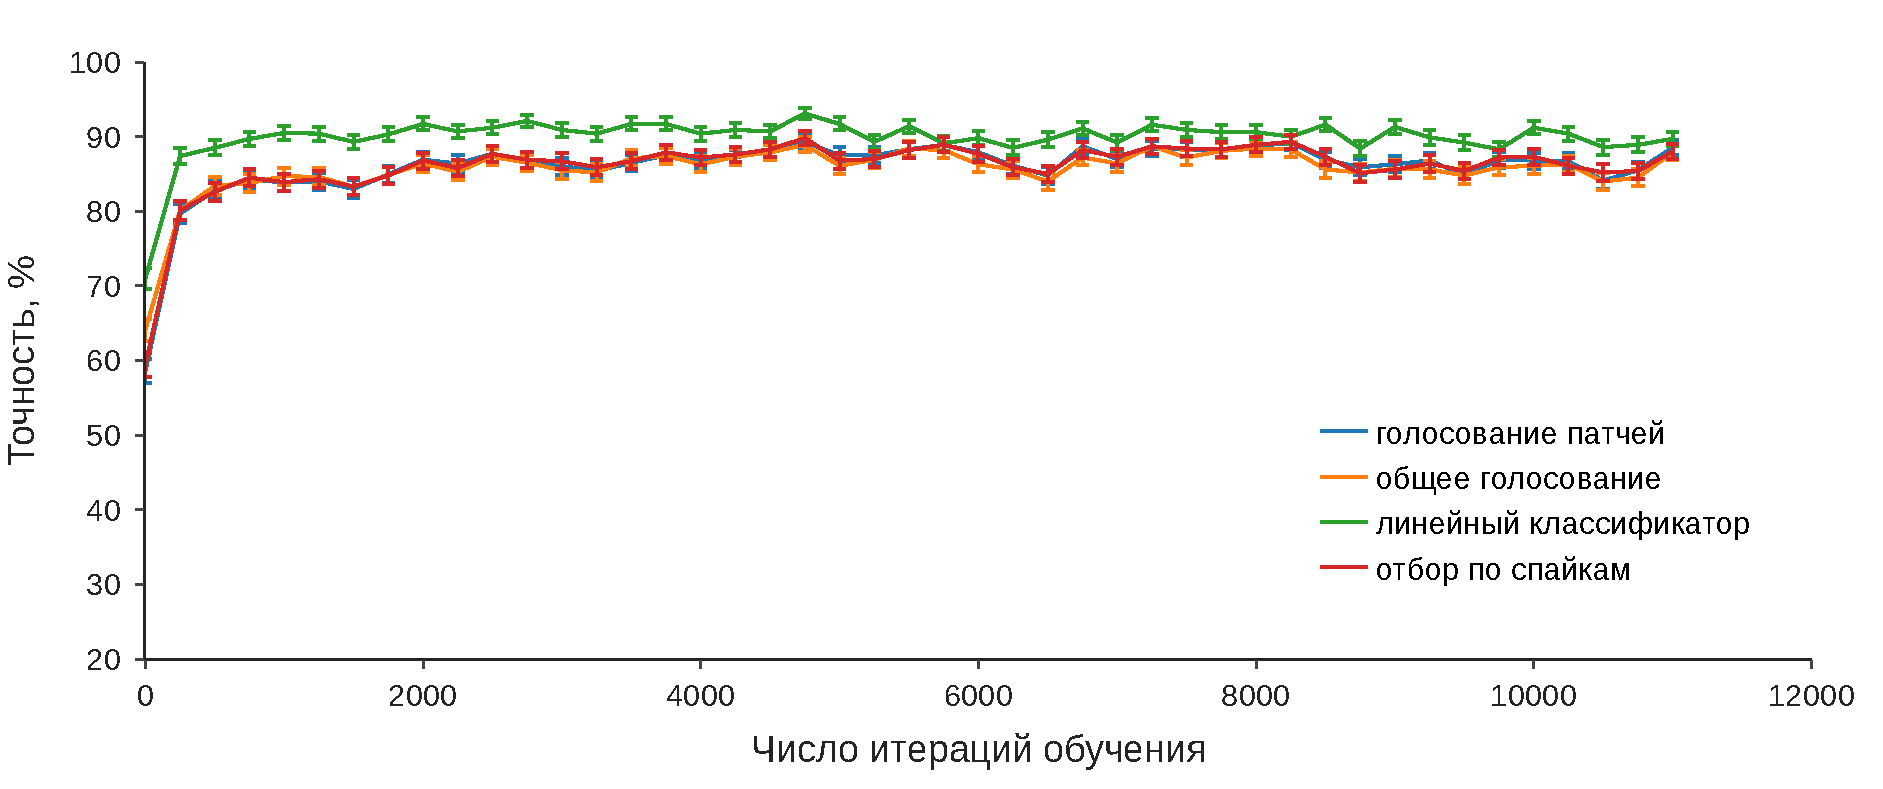
\includegraphics[width=\textwidth,keepaspectratio=true]{LCSNN_learning_rate_ru.pdf}
 \caption{LCSNN learning curve.}
 \label{LCSNN_learning_curve}
\end{subfigure} 
\begin{subfigure}{0.48\textwidth} 
    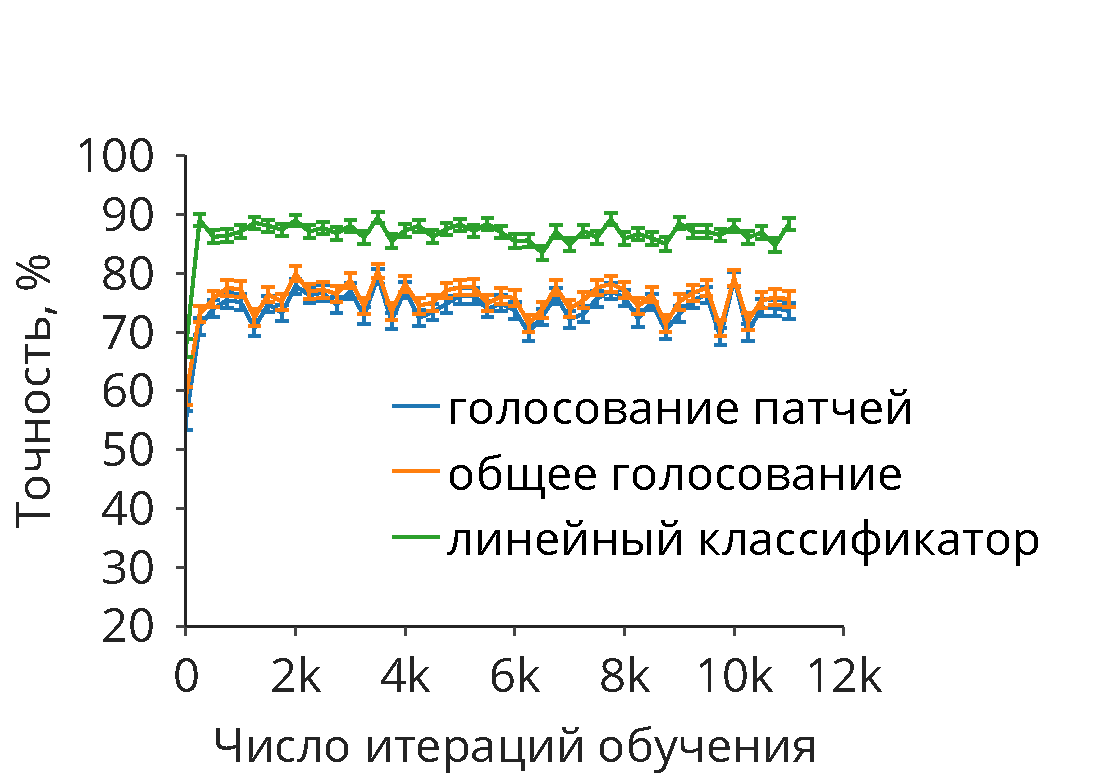
\includegraphics[width=\textwidth,keepaspectratio=true]{CSNN_learning_rate_ru.pdf}
 \caption{CSNN learning curve.}
 \label{CSNN_learning_curve}
\end{subfigure} 
\end{figure}
\begin{figure}\ContinuedFloat
\begin{subfigure}{0.48\textwidth} 
    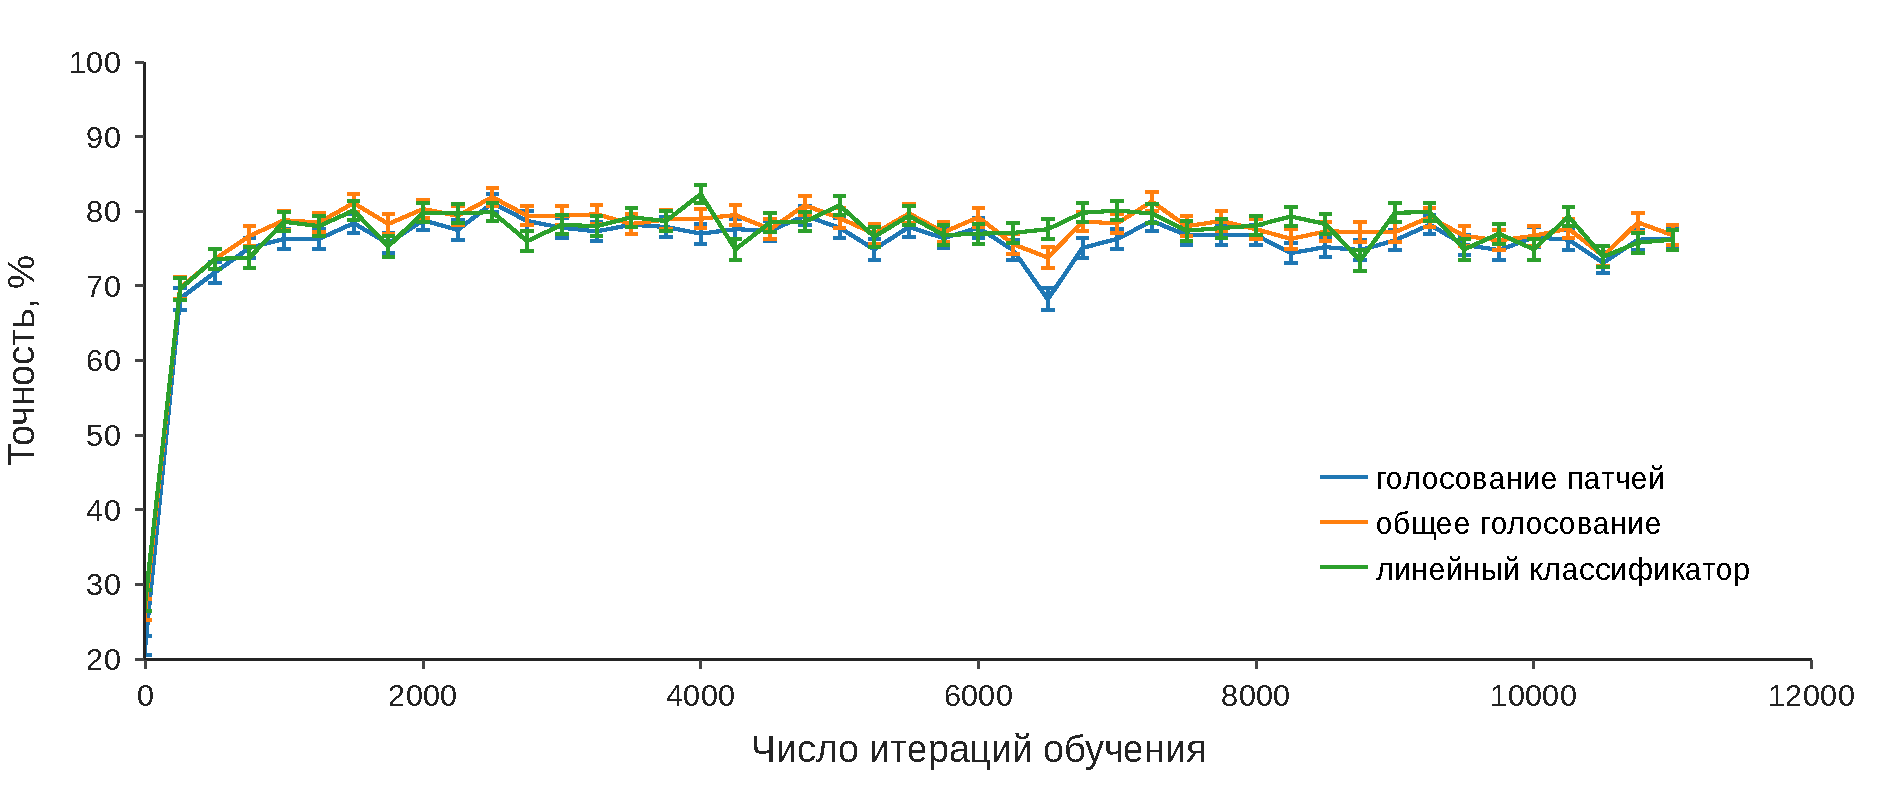
\includegraphics[width=\textwidth,keepaspectratio=true]{FCSNN_learning_rate_ru.pdf}
 \caption{FCSNN learning curve.}
 \label{FCSNN_learning_curve}
\end{subfigure}
\caption{Comparison of learning curves of different architectures of SNNs with competition: (\ref{LCSNN_learning_curve}) LCSNN, (\ref{CSNN_learning_curve}) CSNN, (\ref{FCSNN_learning_curve}) FCSNN. The results are evaluated with different algorithms for the interpretation of activity. The \textbf{preselections by spikes} algorithm was only checked for LCSNN, because it achieves practically same results as \textbf{patch voting}. Standard deviations are plotted as errors. The networks have 100 channels (for a FCSNN the channel consists of a single neuron), the convolution kernel for LCSNN is 12, and for CSNN it is 8.}
\end{figure}

\subsection{Сравнение эффективности операции свертки и локального рецептивного поля}
Были проведены эксперименты по измерению точности сетей с различными архитектурами. Для сверточных и полносвязных сетей вводились аналогичные LCSNN связи конкуренции. Из-за высоких вычислительных нагрузок не ставилось задачи по нахождению параметров, обеспечивающих максимальную точность для каждой архитектуры. Эти параметры были подобраны приблизительно, однако, судя по результатам отдельных отладочных экспериментов, величина расхождения с оптимальными значениями не превышает 1-2\%. Заметим, что при использовании линейного классификатора в качестве алгоритма интерпретации удалось достигнуть 95\% точности для локально соединенной сети из 1000 каналов с размером ядра 12.


\begin{table}
 \caption{Результаты сравнения различных архитектур спайковых нейронных сетей. Для каждой конфигурации точность измерялась $N=5$ раз. В таблице указаны среднее арифметическое значение точности и его стандартное отклонение. <<Ядро>> соответсвует числу $k$ в размере свертки $k\times k$.}
\begin{center}
\begin{adjustwidth}{-1cm}{}
\begin{tabular}{|l|l|l|l|l|l|p{2.2cm}|p{2.2cm}|}
\hline
&\multicolumn{5}{c|}{Конфигурация} & \multicolumn{2}{c|}{Точность, \%}\\
\hline
N & Архитектура & Каналы & Ядро & Параметры & $Y$ нейроны & {Метод \footnotemark[1]} & {Метод \footnotemark[2]} \\
\hline\hline
{\textbf{1}} & {\textbf{LCSNN}} & {\textbf{1000}} & {\textbf{12}} & {\textbf{10287000}} & {\textbf{9000}} & {$\mathbf{92.3 \pm 0.7}$} & {$\mathbf{95.1 \pm 0.5}$}\\
\hline
2 & {LCSNN} & {100} & {12} & {218700} & {900} & {$87.5 \pm 0.9$} & {$91.5 \pm 0.6$}\\
\hline
3 & {LCSNN} & {100} & {8} & {260800} & {1600} & {$82.9 \pm 0.6$} & {$88.1 \pm 0.7$}\\
\hline
{\textbf{4}} & {\textbf{LCSNN\footnotemark[3]}} & {\textbf{25}} & {\textbf{12}} & {\textbf{37800}} & {\textbf{225}} & {$\mathbf{82.3 \pm 1.0}$} & {$\mathbf{88.2 \pm 0.6}$}\\
\hline
5 & {LCSNN} & {25} & {12} & {37800} & {225} & {$80.1 \pm 1.0$} & {$85.5 \pm 0.8$}\\
\hline
6 & {LCSNN} & {25} & {8} & {35200} & {400} & {$73.6 \pm 1.0$} & {$80.3 \pm 0.7$}\\
\hline\hline
7 & {CSNN} & {169} & {12} & {279864} & {1521} & {$79.2 \pm 1.6$} & {$85.7 \pm 1.4$}\\
\hline
8 & {CSNN} & {81} & {12} & {69984} & {729} & {$77.2 \pm 1.7$} & {$83.1 \pm 1.2$}\\
\hline
9 & {CSNN} & {100} & {8} & {164800} & {1600} & {$77.4 \pm 1.9$} & {$82.1 \pm 1.3$}\\
\hline
10 & {CSNN} & {25} & {12} & {9000} & {225} & {$65.8 \pm 0.7$} & {$77.1 \pm 0.6$}\\
\hline
11 & {CSNN} & {25} & {8} & {11200} & {400} & {$63.1 \pm 1.2$} & {$75.8 \pm 0.5$}\\
\hline\hline
12 & {FCSNN} & {100} & {20} & {49900} & {100} & {$81.4 \pm 0.9$} & {$82.1 \pm 0.8$}\\
\hline
\end{tabular}
\end{adjustwidth}
\end{center}
 \label{results}
\end{table}

\footnotetext[1]{Лучший алгоритм голосования}
\footnotetext[2]{Линейный классификатор}
\footnotetext[3]{Сеть с обучением связей конкуренции}

Видно (№2 и №7 в таблице \ref{results}), что локально соединенная сеть превосходит сверточную сеть по точности даже при чуть превышающем числе параметров последней. Также, можно заметить, что не следует использовать слишком малый размер ядра свертки. Это приводит к выучиванию менее существенных признаков. Действительно, в традиционном машинном обучении на основе ИНН используются либо неглубокие сети с большими ядрами свертки, либо глубокие модели, но, наоборот, с маленькими ядрами свертки.

Следует отметить, что SNN могут достигать значительно больших точностей распознавания на MNIST. Для этого можно использовать: (i) cети с существенно большим числом весовых параметров (например, с увеличенным числом каналов); (ii) более глубокие сети (с большим количеством слоев); (iii) более эффективные на сегодня алгоритмы обучения (например, обучение с учителем или с использованием контрастивной функции потерь \cite{contrastive_loss}). В то же время, достижение максимально возможной точности не являлось целью настоящего исследования, адресованного, в первую очередь, сравнению различных архитектур SNN.

\begin{table}
 \caption{Результаты других исследований спайковых нейронных сетей. Во всех используется датасет MNIST.}
\begin{center}
\begin{tabular}{|l|p{4cm}|p{7cm}|l|l|}
\hline
Статья & Архитектура & Обучение & Точность, \% \\
\hline\hline
{Эта работа} & {Локальная + конкуренция} & {Без учителя} & {$95.1 \pm 0.5$}\\
\hline\hline
{\cite{saunders2019locally}} & {Локальная + конкуренция} & {Без учителя} & {$95.07 \pm 0.63$}\\
\hline
{\cite{mnist2}} & {Полносвязная + конкуренция} & {Без учителя} & {95}\\
\hline
{\cite{MaxActiv1}} & {Полносвязная + конкуренция} & {С учителем / с частичным привлечением учителя} & {95.4 / 72.1}\\
\hline
{\cite{conv1}} & {Сверточная} & {С частичным привлечением учителя} & {$96.95 \pm 0.08$}\\
\hline
{\cite{conv2}} & {Сверточная} & {С частичным привлечением учителя} & {$99.28 \pm 0.10$}\\
\hline
{\cite{conv3}} & {Сверточная} & {С частичным привлечением учителя} & {$97.20 \pm 0.07$}\\
\hline
\end{tabular}
\end{center}
\end{table}

Результат, полученный в настоящей работе, практически соответствует результату из \cite{saunders2019locally}. Заметим, что при помощи признаков, обученных без учителя достигаются результаты, лишь немногим уступающие результатам, полученным при помощи обучения с учителем. При этом лучшая локально соединенная сеть с конкуренцией локальных рецептивных полей из этой работы имеет $10^7$ связей (из них связей прямого распространения --- $1 \cdot 10^6$, связей конкуренции --- $9 \cdot 10^6$), по сравнению с $4.6 \cdot 10^7$ (из них связей прямого распространения --- $0.5 \cdot 10^7$, связей конкуренции --- $4.1 \cdot 10^7$) у полносвязной сети с конкуренцией из \cite{mnist2}. К тому же, обучение сети из \cite{mnist2} велось в течение $1 \cdot 10^6$ итераций, тогда как в этой работе число итераций обучения не превосходит 5000.

\section{Обучение связей конкуренции}
Ингибирующие связи $YY$ существенно влияют на обучение связей прямого распространения сигнала $XY$. Большие по модулю значения весов конкуренции способствуют большей вариативности и специализации в обучении $Y$ нейронов, так как для каждого рецептивного поля одновременно активными не могут быть нейроны, имеющие схожие веса $XY$ (Рис. \ref{fig:high_comp}). Наоборот, малые по модулю веса конкуренции не позволяют нейронам эффективно специализироваться (Рис. \ref{fig:high_comp}).

\begin{figure}
\centering
\begin{subfigure}{0.45\textwidth}
    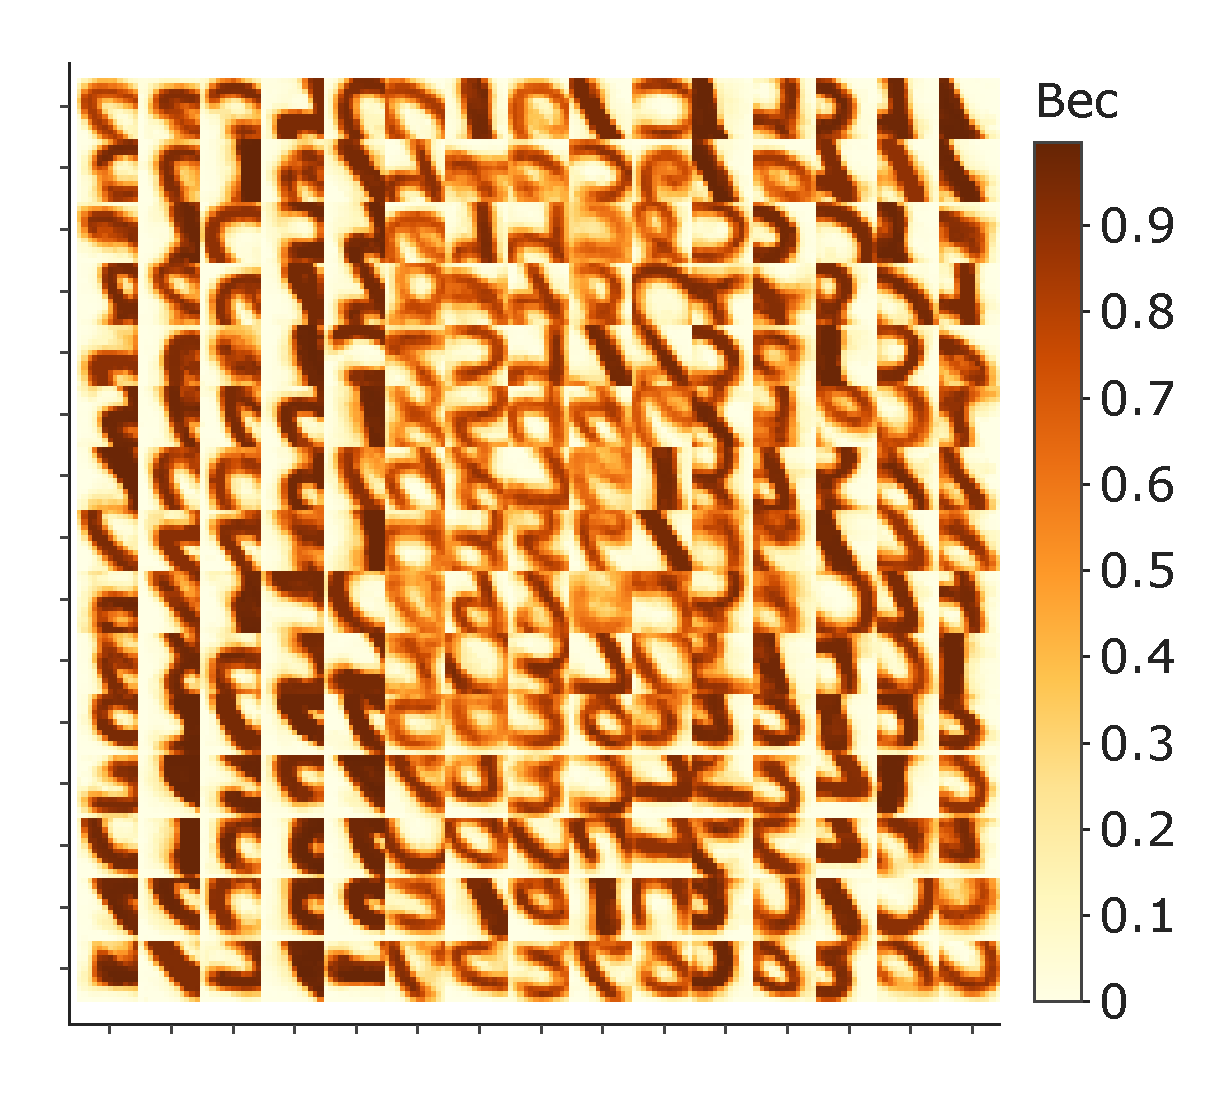
\includegraphics[width=\textwidth,keepaspectratio=true]{weights_XY_good_ru.pdf}
    \caption{Высоко специализированные веса, вес конкуренции равен --100.}
    \label{fig:high_comp}
\end{subfigure}
\begin{subfigure}{0.45\textwidth}
    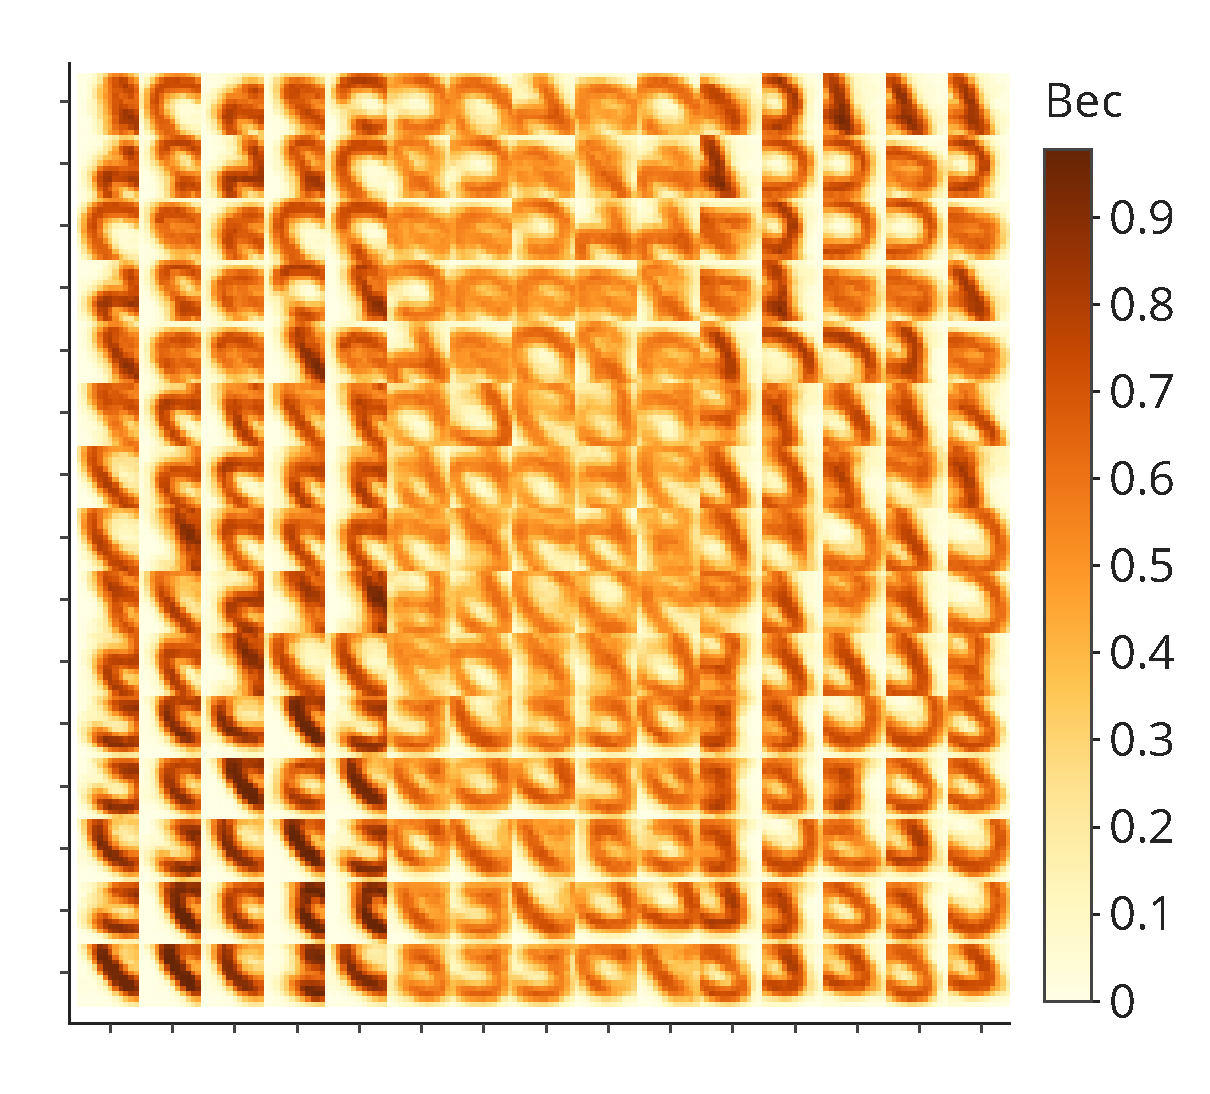
\includegraphics[width=\textwidth,keepaspectratio=true]{weights_XY_bad_ru.pdf}
    \caption{Слабо специализированные веса,\\ вес конкуренции равен --10.}
    \label{fig:low_comp}
\end{subfigure}
\caption{Влияние конкуренции на обучение связей $XY$.}
\label{competition-training-importance}
\end{figure}

Все SNN, о которых шла речь в настоящей работе до этого момента, имели фиксированные веса конкуренции. В связи с этим, возникает вопрос, как влияет на точность сети обучение весов конкуренции. Для ответа на поставленный вопрос с целью обновления связей $YY$ было выбрано правило anti-STDP (правило, противоположное по знакам $A_{+}$ и $A_{-}$ в стандартном STDP). При варьировании значений параметров этого правила были получены различные распределения весов конкуренции. Начальные значения весов конкуренции задавались из равномерного распределения от 0 до некоторого числа, которое в дальнешем будем называть начальным весом конкуренции. Эксперименты проводились с LCSNN.

\begin{table}
 \caption{Параметры anti-STDP}
\begin{center}
\begin{tabular}{|l|l|l|l|l|}
\hline
Рисунок & {$\tau_{+}$, мс} & {$\tau_{-}$, мс} & {$A_{+}$} & {$A_{-}$} \\
\hline
\ref{fig:worst_competition_distribution} & 14.7 & 14.2 & -0.5 & -1.5 \\
\hline
\ref{fig:medium_bad_competition_distribution} & 5.4 & 15.1 & -1.2 & -0.6 \\
\hline
\ref{fig:medium_good_competition_distribution} & 17.6 & 24.5 & -1.9 & -1.6 \\
\hline
\ref{fig:best_competition_XY} & 17.7 & 16.5 & -0.1 & -1.6\\
\hline
\end{tabular}
\end{center}
\end{table}

\begin{figure}
\centering
\begin{subfigure}{0.45\textwidth}
    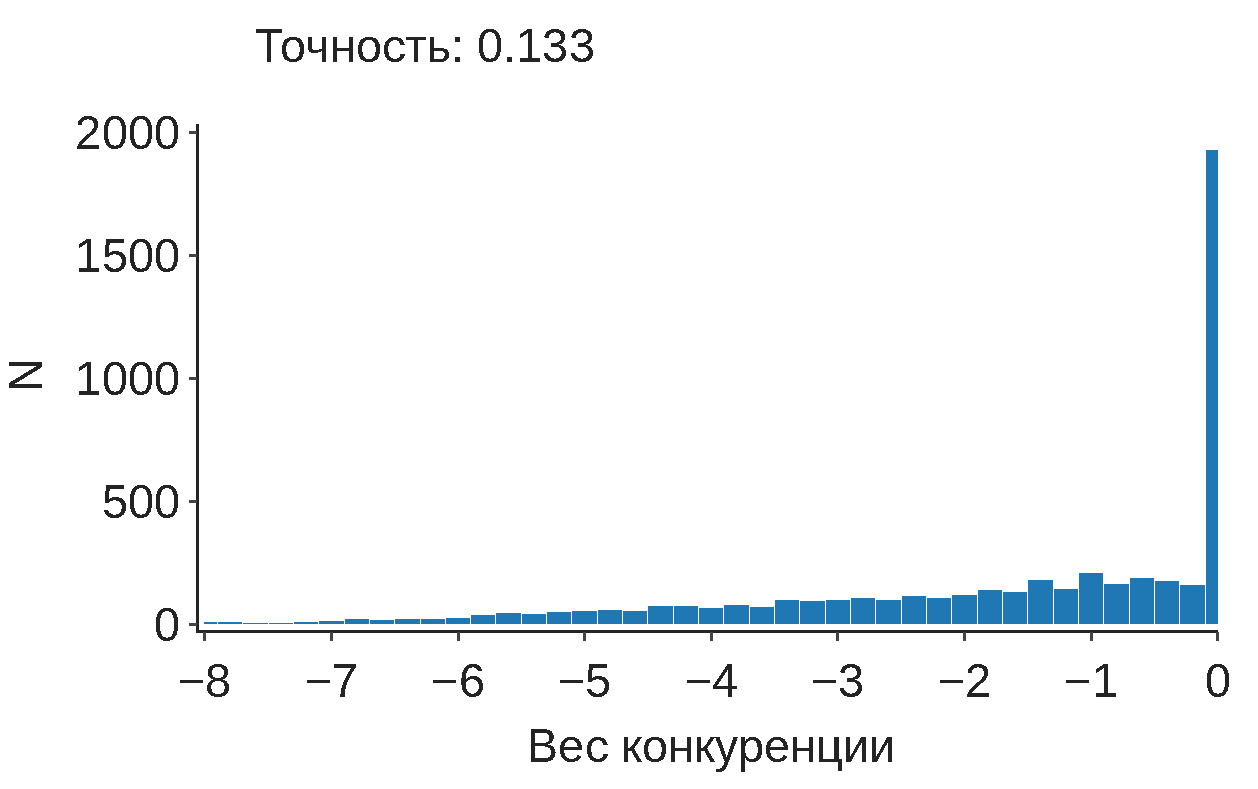
\includegraphics[width=\textwidth,keepaspectratio=true]{competition_distribution_worst_ru.pdf}
    \caption{Очень слабая конкуренция}
\end{subfigure}
\begin{subfigure}{0.45\textwidth}
    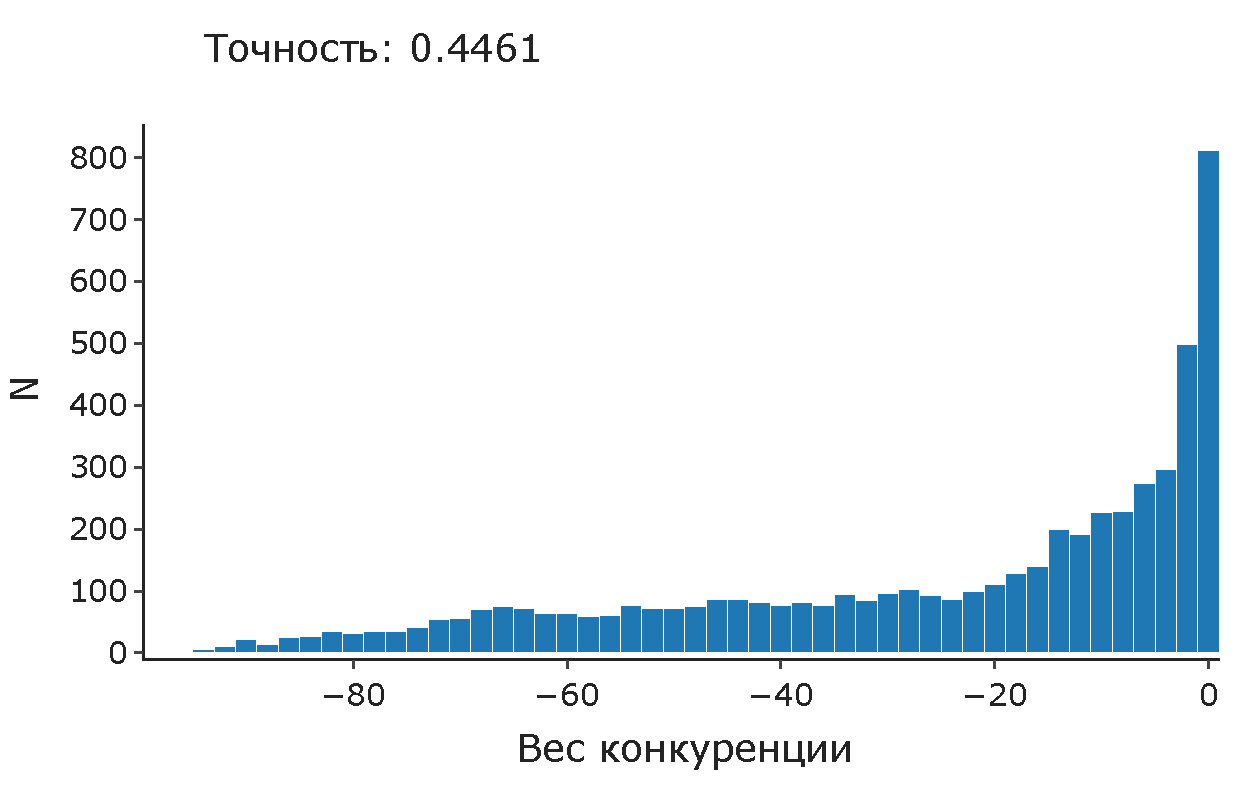
\includegraphics[width=\textwidth,keepaspectratio=true]{competition_distribution_medium_bad_ru.pdf}
    \caption{Слабая конкуренция}
\end{subfigure}
\\
\begin{subfigure}{0.45\textwidth}
    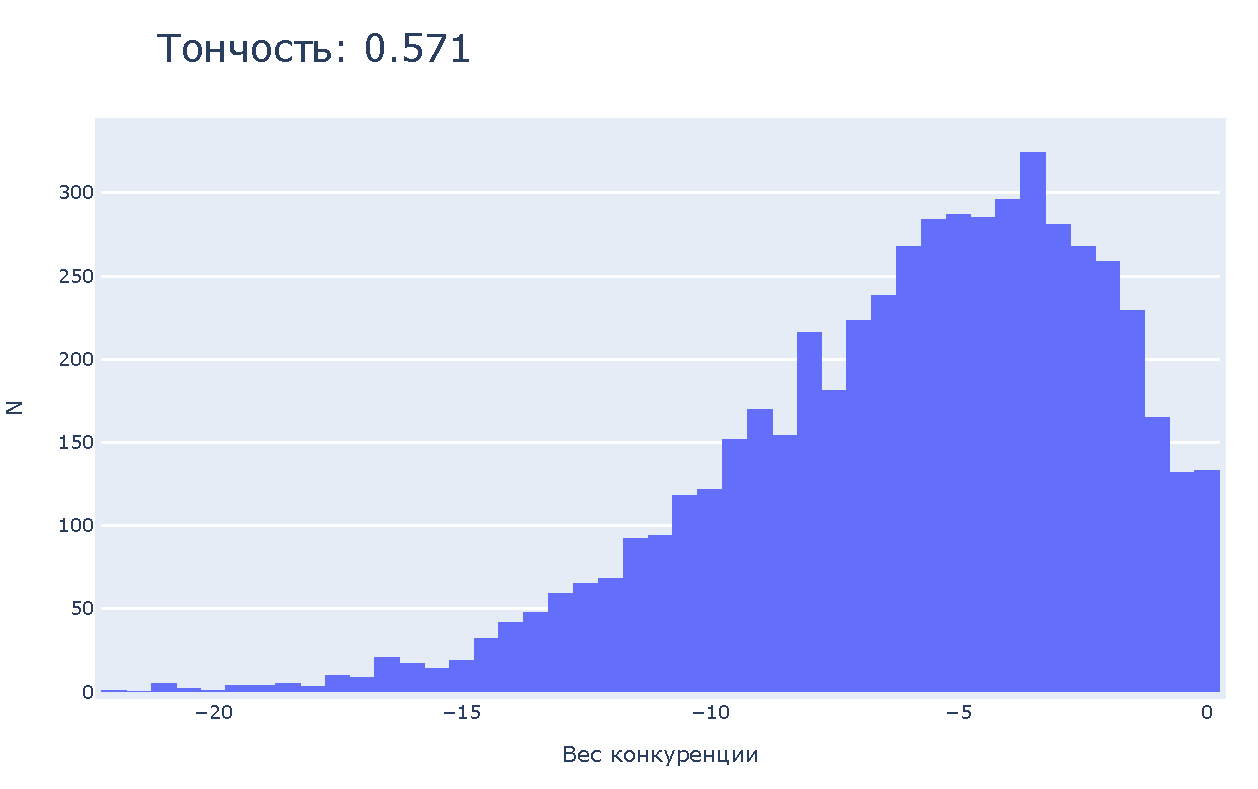
\includegraphics[width=\textwidth,keepaspectratio=true]{competition_distribution_medium_good_ru.pdf}
    \caption{Средняя конкуренция} 
\end{subfigure}
\begin{subfigure}{0.45\textwidth}
    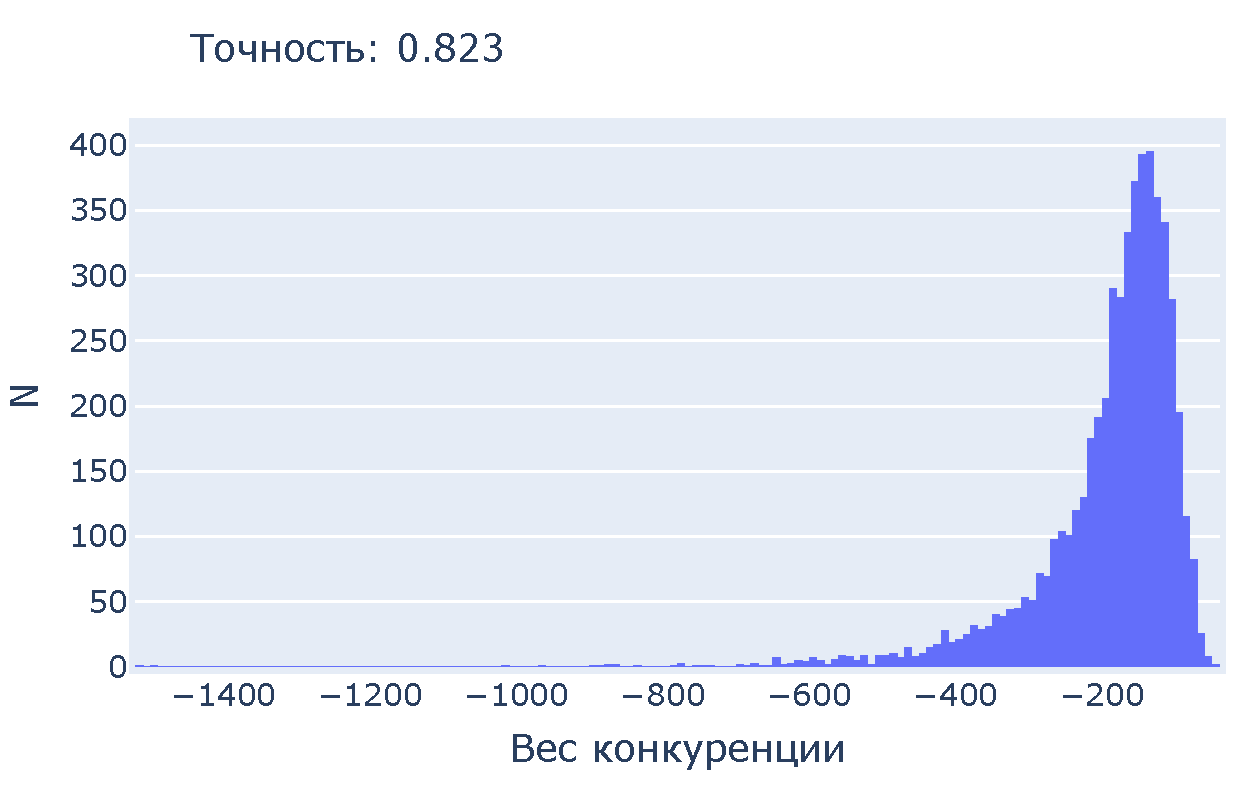
\includegraphics[width=\textwidth,keepaspectratio=true]{competition_distribution_best_ru.pdf}
    \caption{Сильная конкуренция}
    \label{fig:best_competition}
\end{subfigure}
\caption{Различные распределения весов конкуренции}
\label{fig:competition_distributions}
\end{figure}

Видно, что точность сети повышается при смещении распределения весов конкуренции в сторону больших по модулю отрицательных значений. Заметим опять, что целью являлось не нахождение параметров сети, обеспечивающих максимальную точность, а исследование влияния способности обучения конкуренции на точность сети с заданной конфигурацией остальных параметров.

Примечательно, что не все связи $YY$ получают большие по модулю значения (Рис. \ref{fig:best_competition}). Это объясняется тем, что нейроны, специализирующиеся на существенно разных признаках, не нуждаются в конкуренции, так как они не проявляют высокую активность одновременно.

\begin{figure}
\centering
\begin{subfigure}{0.45\textwidth} 
    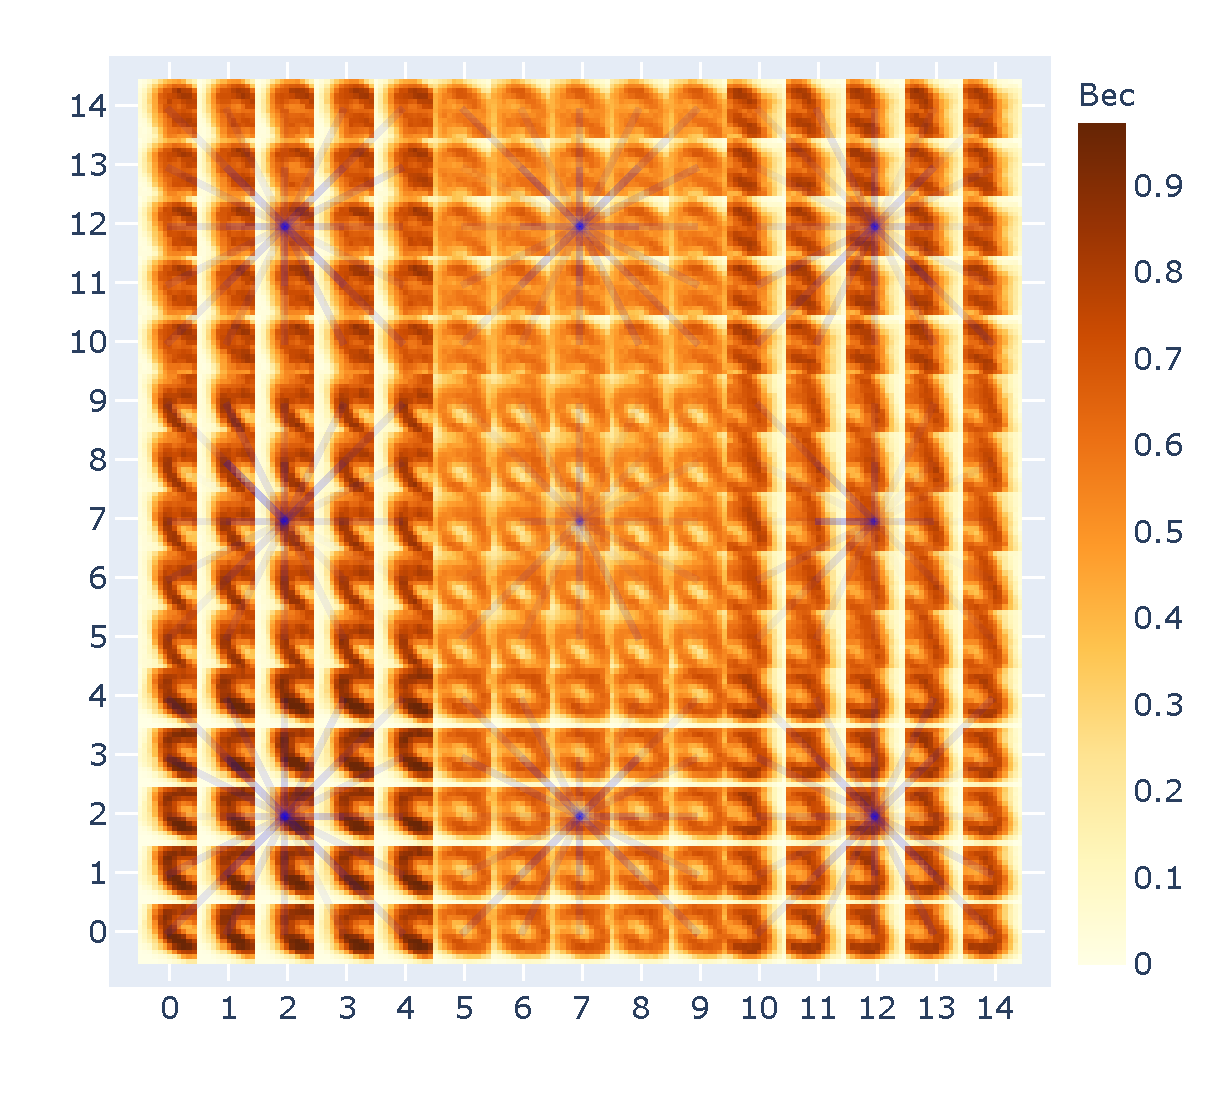
\includegraphics[width=\textwidth,keepaspectratio=true]{competition_on_XY_worst_ru.pdf}
    \caption{Очень слабая конкуренция}
    \label{fig:worst_competition_distribution}
\end{subfigure}
\begin{subfigure}{0.45\textwidth}
    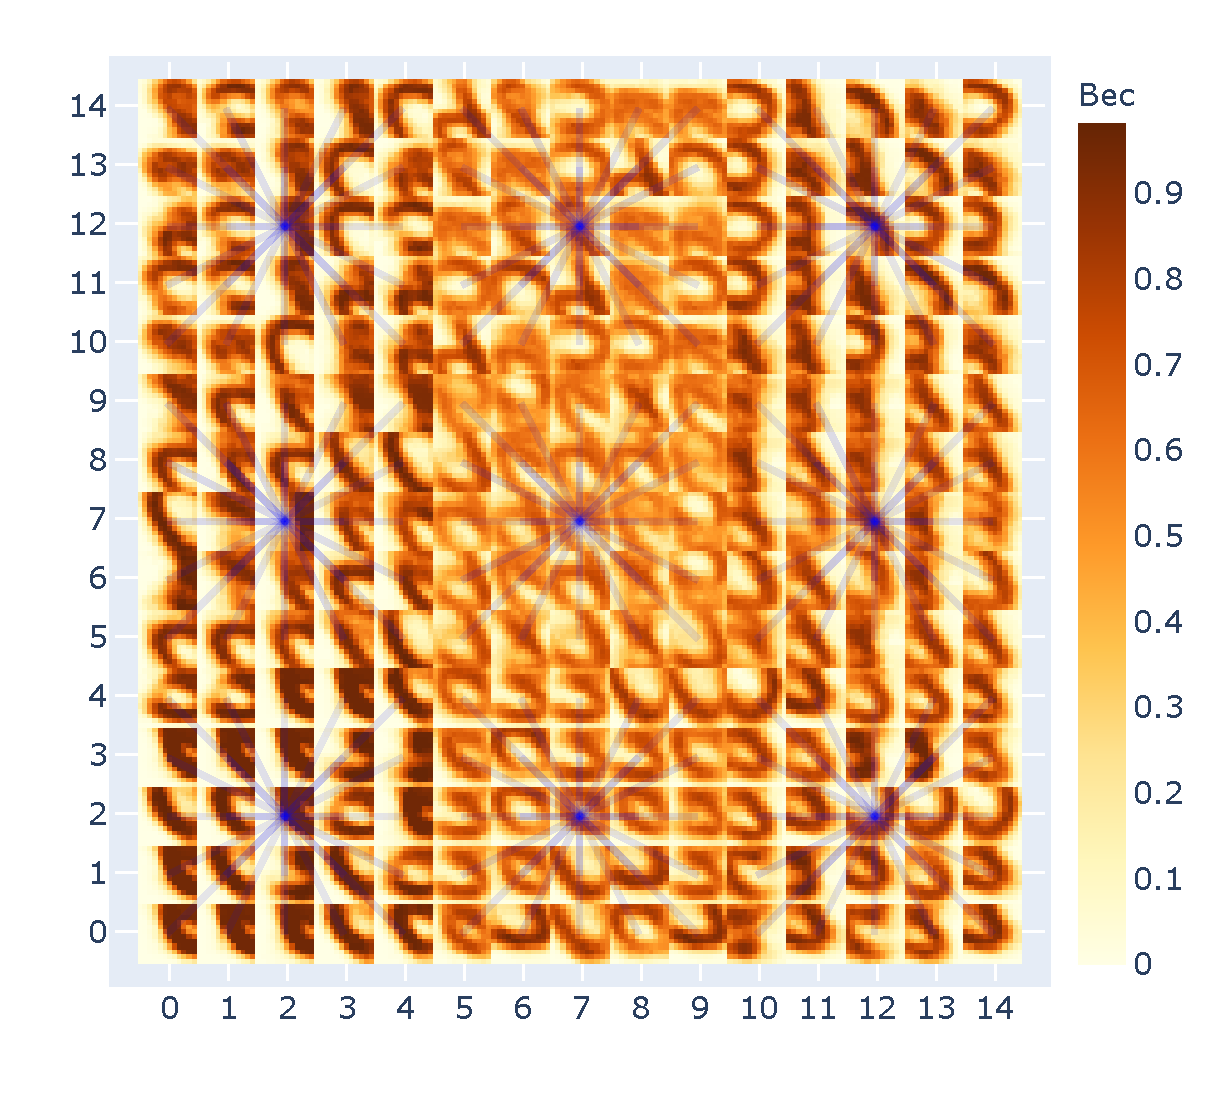
\includegraphics[width=\textwidth,keepaspectratio=true]{competition_on_XY_medium_bad_ru.pdf}
    \caption{Слабая конкуренция}
    \label{fig:medium_bad_competition_distribution}
\end{subfigure}
\\
\begin{subfigure}{0.45\textwidth}
    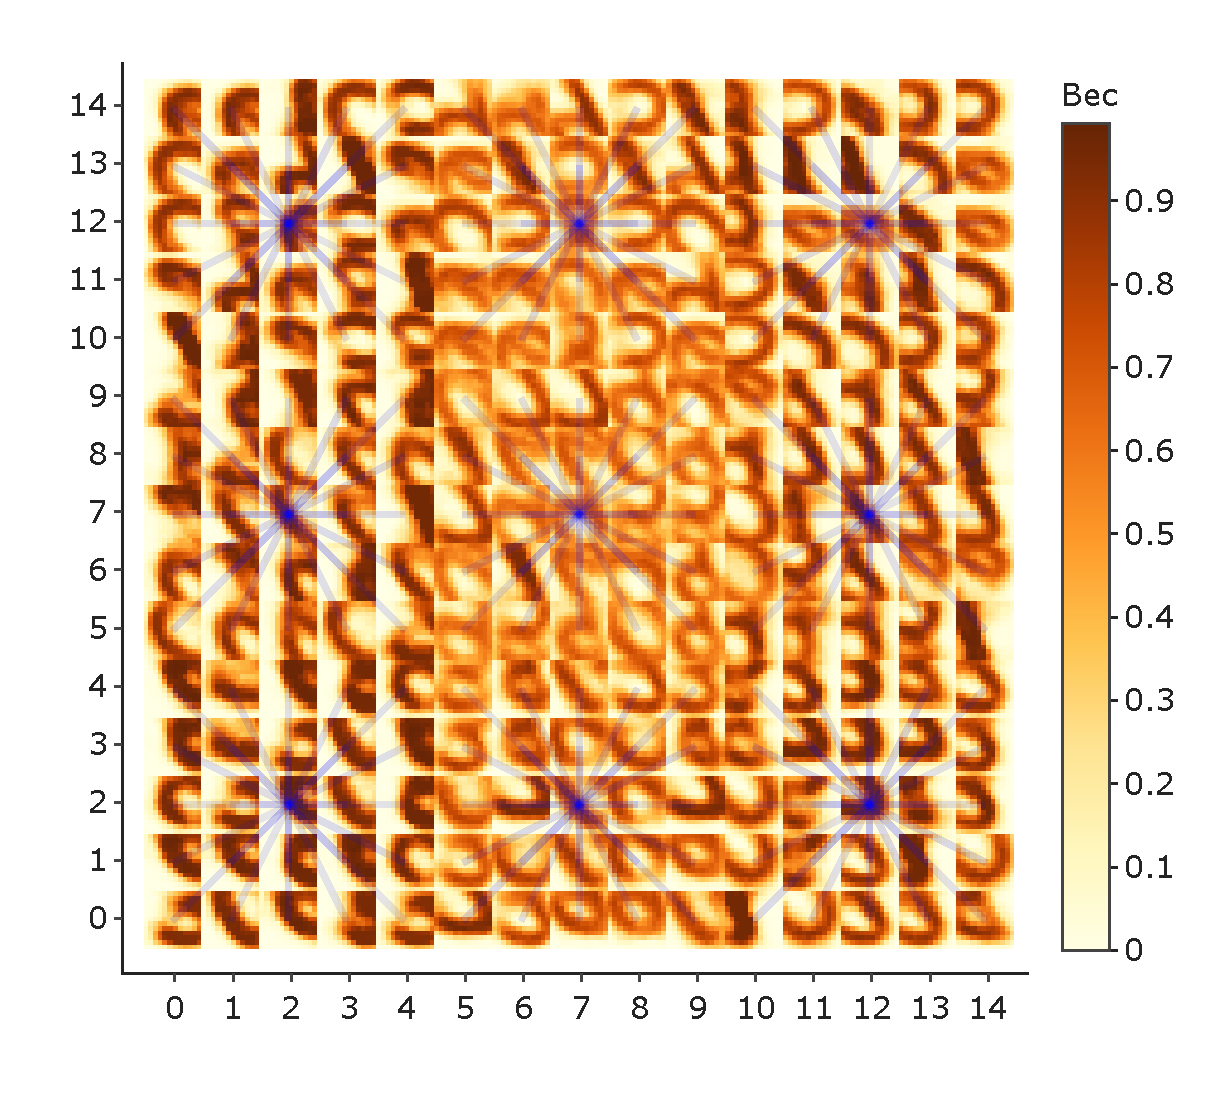
\includegraphics[width=\textwidth,keepaspectratio=true]{competition_on_XY_medium_good_ru.pdf}
    \caption{Средняя конкуренция}
    \label{fig:medium_good_competition_distribution}
\end{subfigure}
\begin{subfigure}{0.45\textwidth} 
    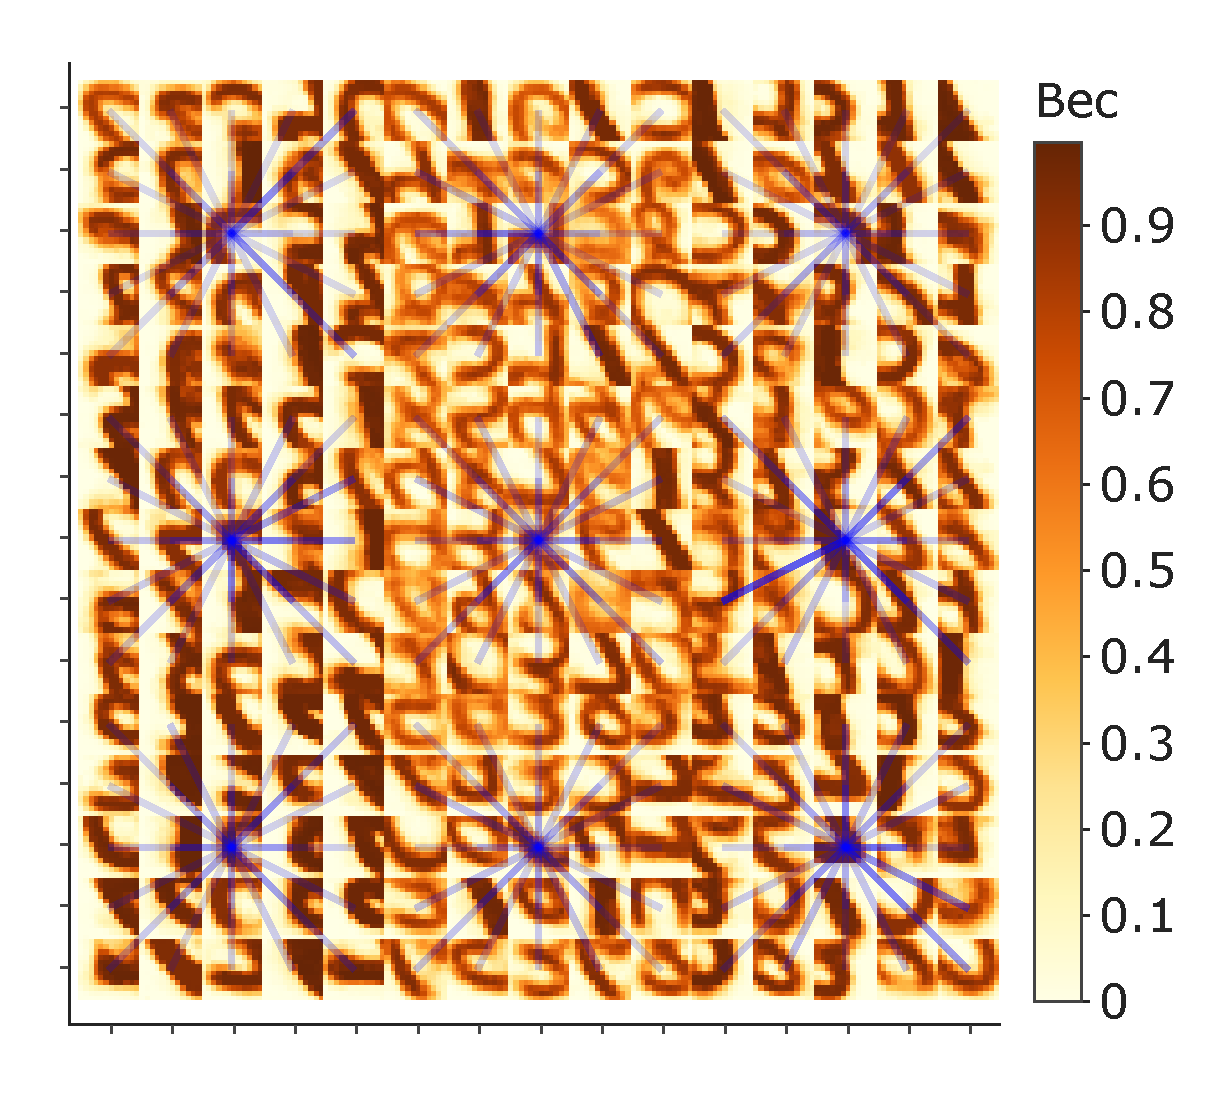
\includegraphics[width=\textwidth,keepaspectratio=true]{competition_on_XY_best_ru.pdf}
    \caption{Сильная конкуренция}
    \label{fig:best_competition_XY}
\end{subfigure}
\caption{Визуализация весов конкуренции поверх весов $XY$. Изображения соответствуют весам сетей с рисунка \ref{fig:competition_distributions}. Изображены только веса конкуренции для одного нейрона в каждом рецептивном поле для избегания загромождения визуализации. Насыщенный синий цвет соответствует большим по модулю весам конкуренции (используется среднее арифметическое между весами $W_{ij}$ и $W_{ji}$). Видно, что похожие признаки сильнее конкурируют между собой, чем различные.}
\end{figure} 

Обучение конкуренции производилось только на сетях из 25 каналов (225 нейронов), так как его моделирование требует больших вычислительных ресурсов.

В ходе оптимизации моделей была измерена точность большого количества LCSNN с различными конфигурациями гиперпараметров (Рис. \ref{fig:hyperparams}). Видно, что конфигурации с высокими точностями (темные ломаные) локализуются определенным образом - дописать

\begin{figure}
\begin{center}
 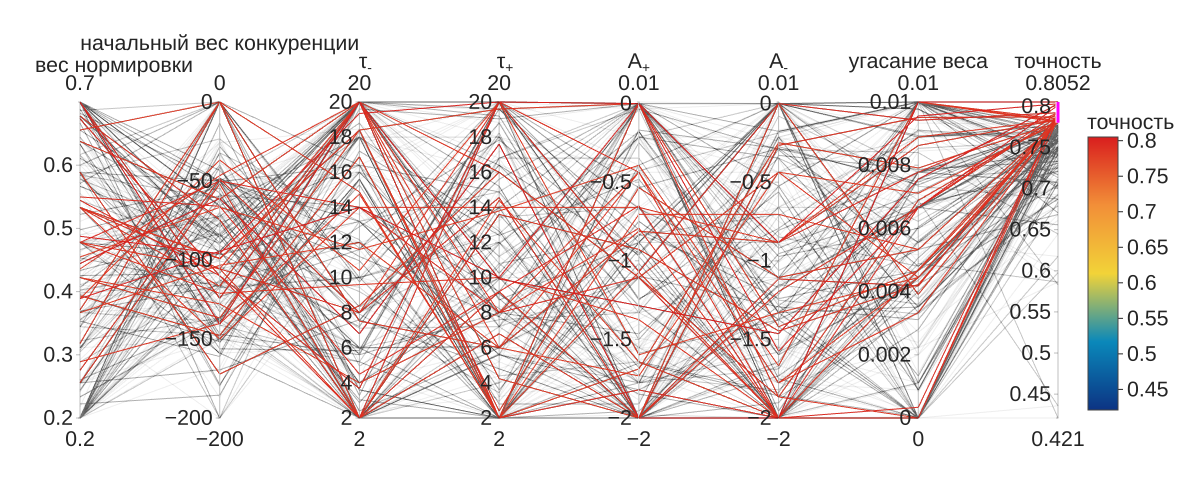
\includegraphics[,
 width=\textwidth,keepaspectratio=true]{hyperparams_ru.png}
 
\caption{Визуализация достигаемой точности распознавания LCSNN при использовании различных комбинаций параметров в пространстве гиперпараметров. Параметры <<вес нормировки>>, <<начальный вес конкренции>> и <<угасание веса>> отвечают за значения весов, а следующие два являются комбинациями параметров anti-STDP. На последней оси указана точность сети с конфигурацией, соответствующих точкам пересечения ломаной осей гиперпараметров.}
 \label{fig:hyperparams}
\end{center} 

\end{figure}

\subsection{Анализ обученных весов конкуренции}
Дополнительно были проведены эксперименты по ограничению значений весов конкуренции по модулю сверху и снизу до проведения обучения сети. Оказалось, что веса конкуренции во всем диапазоне их изменения играют важную роль в работе LCSNN, поскольку ограничение как сверху, так и снизу негативно влияет на точность распознавания (Рис. \ref{fig:compe_clamp}). Это объясняется тем, что высокая конкуренция способствует большей специализации нейронов и потому полезна, а низкая конкуренция позволяет нейронам кооперироваться и распознавать классы совместно (в том числе обеспечивая накопление большей статистики для калибровки голосов нейронов).

\begin{figure}
\centering 
\begin{subfigure}{0.45\textwidth}
    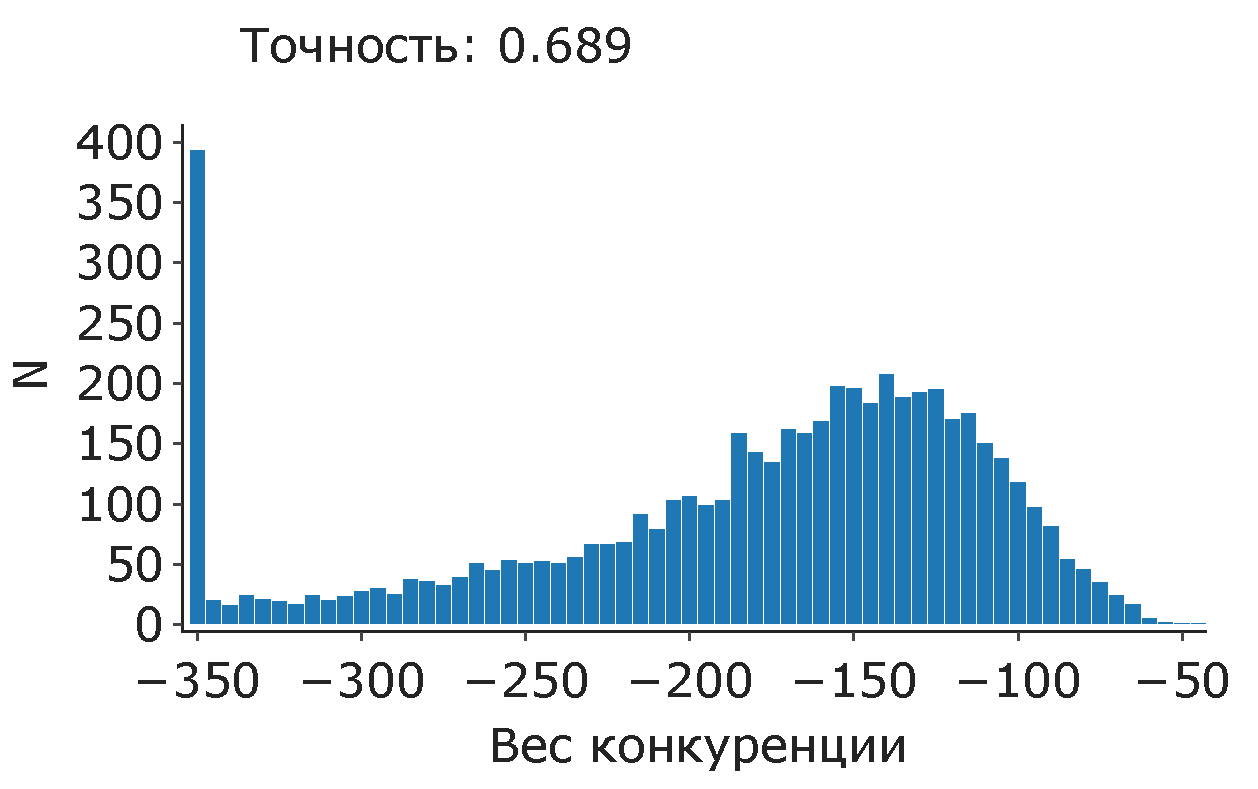
\includegraphics[width=\textwidth,keepaspectratio=true]{competition_distribution_clamp_low_ru.pdf}
    \caption{Распределение весов конкуренции, ограничение сверху} 
\end{subfigure}
\begin{subfigure}{0.45\textwidth}
    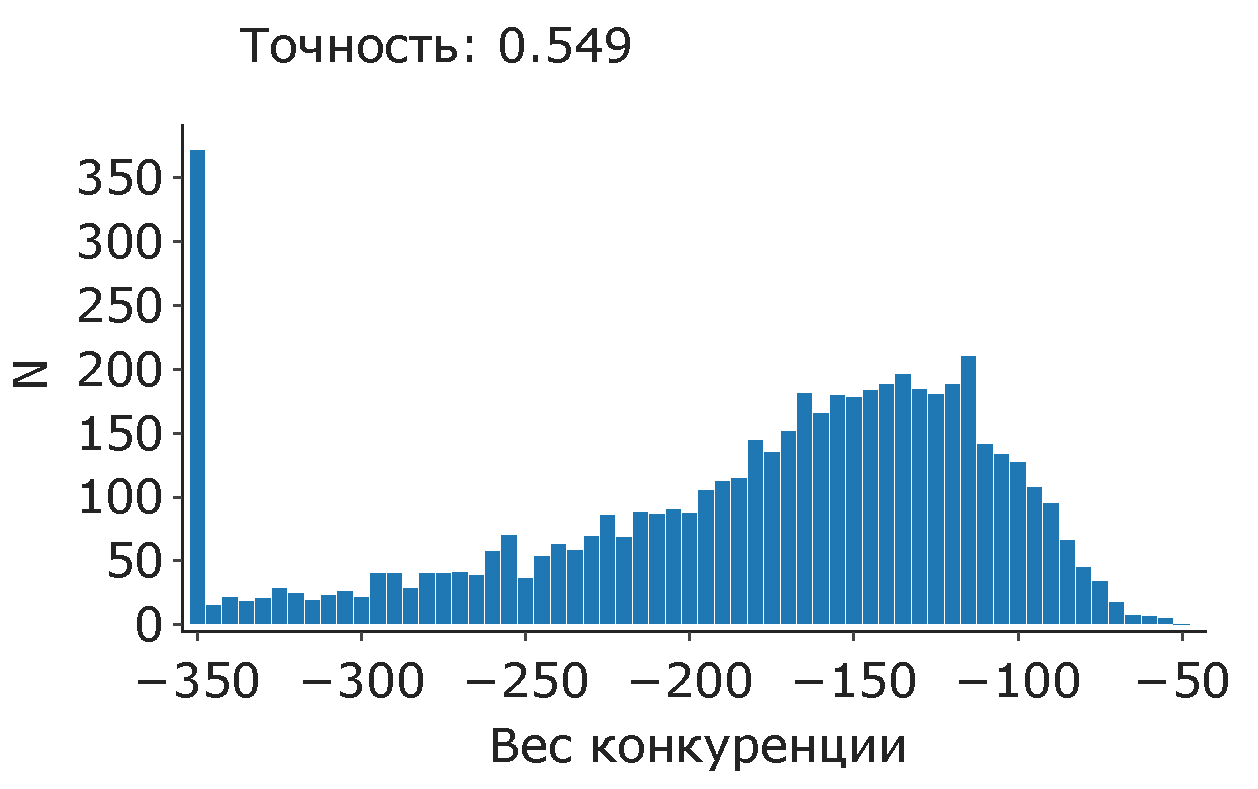
\includegraphics[width=\textwidth,keepaspectratio=true]{competition_distribution_clamp_high_ru.pdf}
    \caption{Распределение весов конкуренции, ограничение снизу}
\end{subfigure}
\begin{subfigure}{0.45\textwidth}
    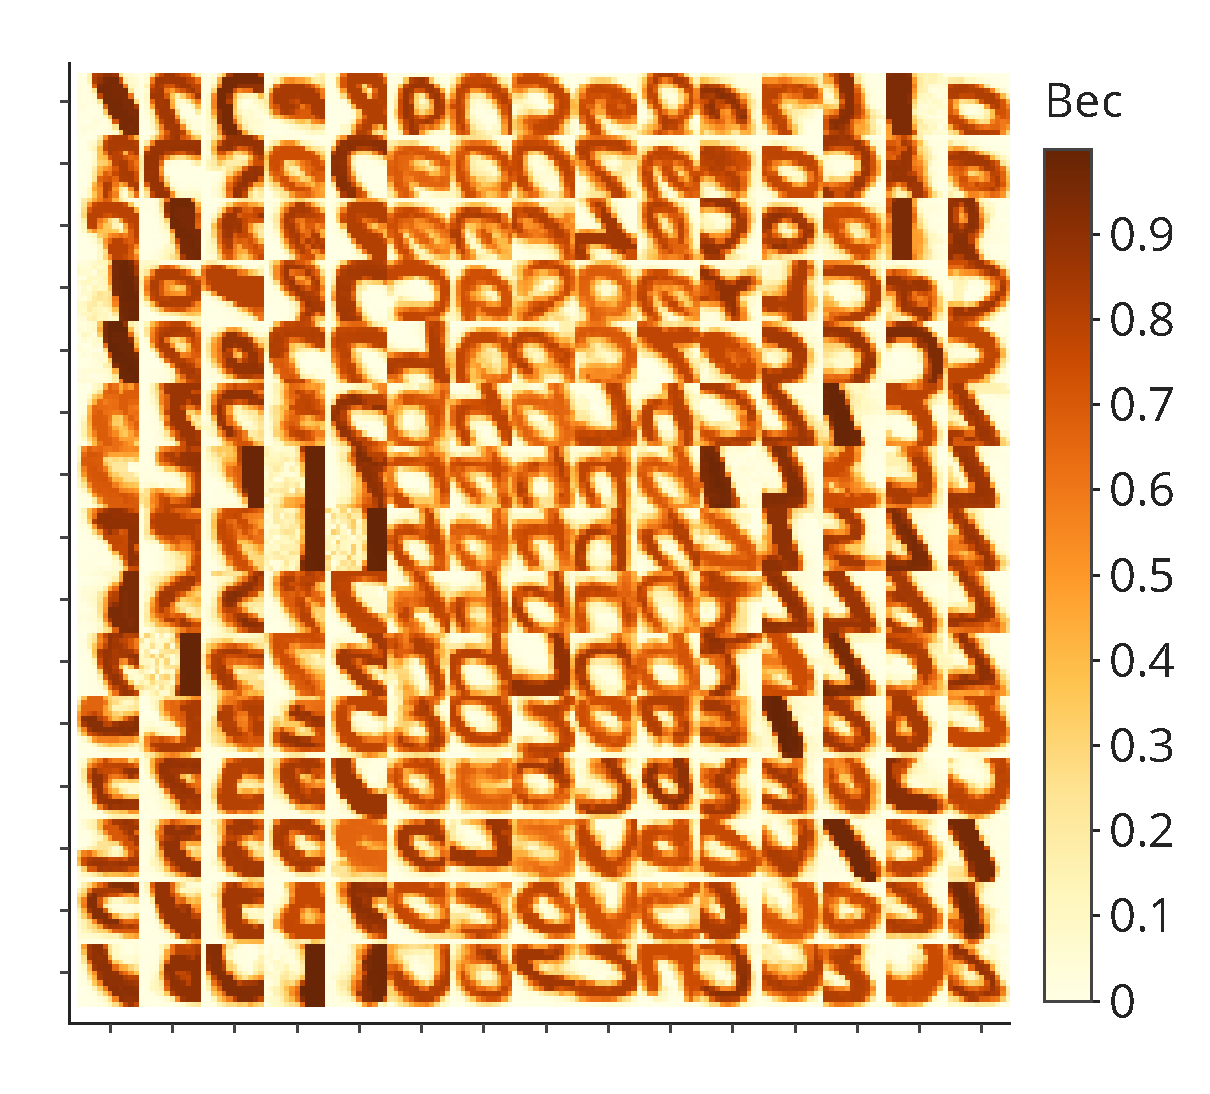
\includegraphics[width=\textwidth,keepaspectratio=true]{weights_XY_clamp_low_ru.pdf}
    \caption{Веса прямого распространения, ограничение сверху}
\end{subfigure} 
\begin{subfigure}{0.45\textwidth}
    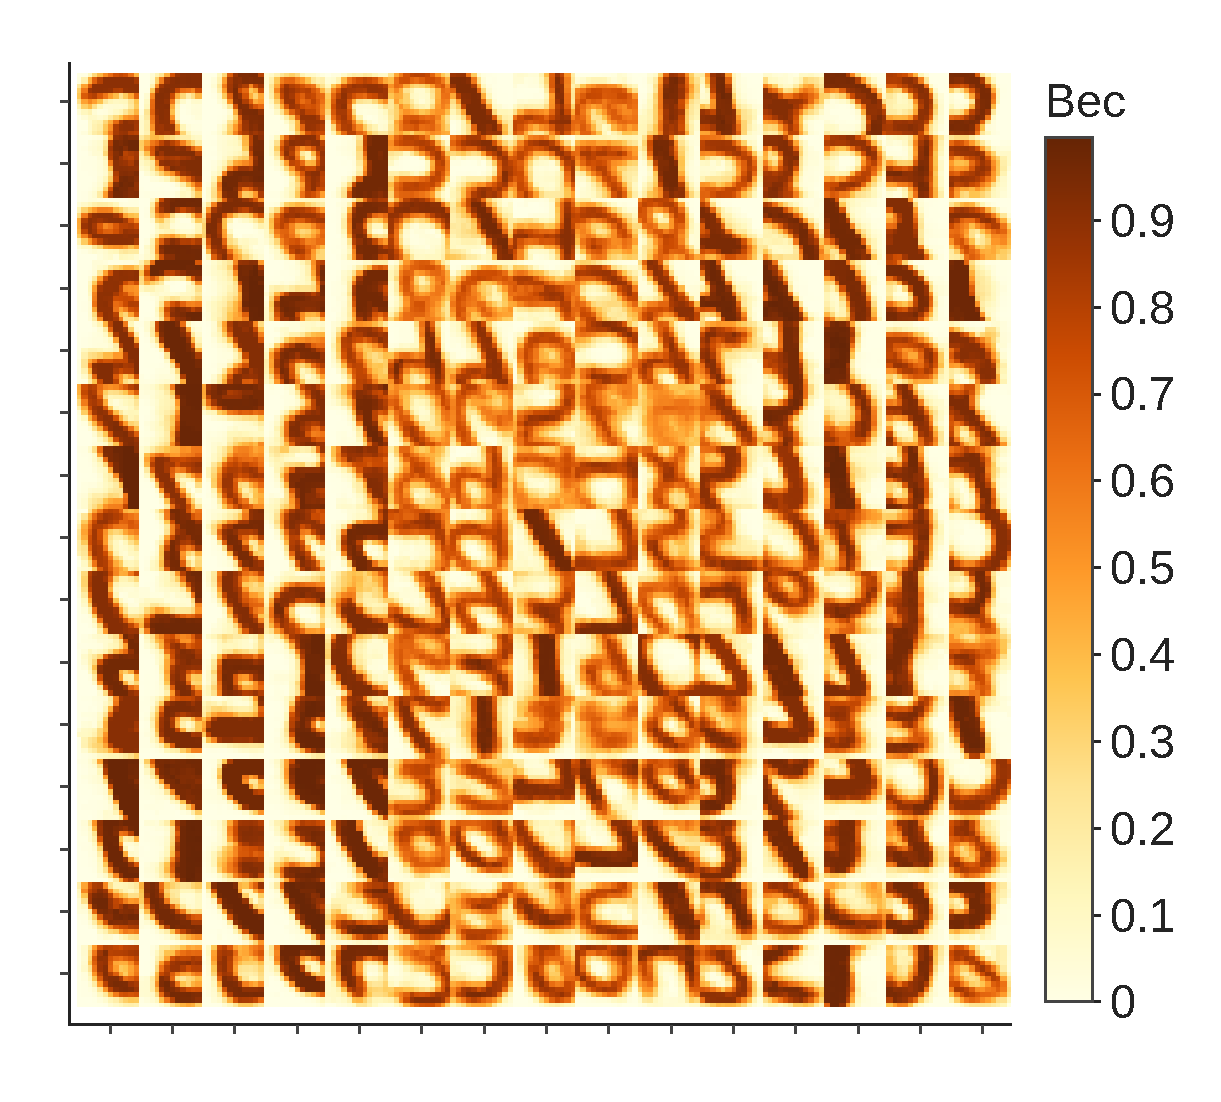
\includegraphics[width=\textwidth,keepaspectratio=true]{weights_XY_clamp_high_ru.pdf}
    \caption{Веса прямого распространения, ограничение снизу}
\end{subfigure} 
\caption{Влияние ограничения значений весов конкуренции на точность. Веса были ограничены значениями $-350$ снизу и $-100$ сверху. Точность сети с аналогичными параметрами, но без ограничения конкуренции составляет 0.823, ее веса $XY$ изображены на Рис. \ref{fig:best_competition_XY}, а распределение ее весов конкуренции --- на Рис. \ref{fig:best_competition}. Видно, что в обоих случаях обучаются менее четкие веса прямого распространения.}
\label{fig:compe_clamp}
\end{figure}

Обучение конкуренции позволило достичь точности, незначительно (на 2\%) превышающей точность сети такой же конфигурации, но с фиксированной конкуренцией с ингибирующими весами, равными $-50$ (Таб. \ref{results}, №4 и №5). 

\section{Обсуждение}
Настоящее исследование демонстрирует, что локально соединенная сеть – перспективная спайковая нейросетевая архитектура, подходящая для эффективной реализации на специализированном нейрочипе. Действительно, способность быстро выходить на плато кривой обучения позволяет использовать LCSNN для обучения на выборках сравнительно небольшого объема (3000-5000). Использование дополнительного алгоритма интерпретации активности, такого как линейный классификатор, позволяет повысить эффективность сети. Заметим, что при этом сами признаки распознаваемых объектов выучиваются сетью без учителя. Остается открытым вопрос о возможности получения схожих результатов без использования обучения с учителем для интерпретации активности сети.

Главным преимуществом LCSNN является, как было показано, то, что локально соединенная сеть превосходит сверточную в точности при примерно одинаковом или чуть большем числе параметров. Предположительно, это происходит за счет более богатой статистики патчей (рецептивных полей), на которые реагируют нейроны внутри каждого канала, по сравнению с одним рецептивным полем на каждый канал в сверточной архитектуре. Ценой за это является увеличенное число параметров в LCSNN, но не является критическим фактором, ввиду локальной (в противоположность полносвязной) топологии межнейронных контактов. Локальная архитектура также позволяет сохранить информацию о локализации выделяемого признака в пространстве и потому является разумным выбором для реализации SNN, обучающихся преимущественно без учителя. Данный выбор обусловливает также его совокупную эффективность (по производимости, точности и энергопотреблению при определённой плотности элементов) при аппаратной реализации, при которой каждый вес обычно представлен одним или несколькими физическими элементами (главным образом, ячейками SRAM \cite{TrueNorth, Loihi} или мемристорами \cite{Li_2018}).
Обучение связей конкуренции слегка увеличивает точность работы алгоритма на базе LCSNN, но не настолько критично, чтобы оправдывать использование такой дорогой операции как введение и обучение значительного числа ингибирующих связей с различными по модулю конечными весами. В то же время, вероятно, этот вывод справедлив только для небольших сетей, вроде исследованной в настоящей работе. На наш взгляд, более тщательного изучения заслуживает подбор оптимальных алгоритмов и параметров обучения конкуренции для глубоких SNN, в которых баланс конкуренции и кооперации нейронов внутри каждого слоя может приводить к формированию кластеров из классов подаваемых изображений, что способствует выстраиванию семантически-подобной иерархии выученных признаков и их комбинаций, то есть конечных образов \cite{10.1007/978-3-030-30425-6_30}. Потенциально такая иерархия образов может привести к существенному приросту качественных показателей работы интеллектуальных алгоритмов. 

\clearpage
\addcontentsline{toc}{section}{Выводы}
\section*{Выводы}
Было показано, что для задачи распознавания образов на датасете MNIST локально соединенная архитектура с конкуренцией превосходит сверточную при равном числе параметров.
Также было показано, что обучение весов конкуренции позволяет незначительно повысить качество модели, а в полученном распределении весов конкуренции важны как высокие по модулю (сильная конкуренция), так и низкие (кооперация) значения весов.


\printbibliography[sorting=none,heading=bibintoc,type=article,title={Литература}]
 
\begin{center}
Все материалы этой работы находятся в репозитории\\
\href{https://github.com/danielgafni/bachelor}{https://github.com/danielgafni/bachelor} 
\end{center}

\end{document}  
